\documentclass[nostrict]{szablonPG}

\usepackage{listing_schemat}

\begin{document}

%\includepdf{meta/strona_tytulowa.pdf}
%\includepdf{meta/oswiadczenie.pdf}

\chapter*{Streszczenie}
Niniejsza praca opisuje proces powstawania projektu pod tytułem: ``Interaktywna wizualizacja stron Wikipedii w jaskini rzeczywistości wirtualnej''. Jest inspirowany Projektem Opte, którego twórcy podjęli próbę zwizualizowania całego internetu, skupia się jednak na mniejszym, bardziej osiągalnym celu: pokazywaniu związków i połączeń między artykułami zamieszczonymi w Wikipedii. 

Po wstępie zostały wyszczególnione wymagania oraz scenariusze użycia tak jak zostały one zdefiniowane przed rozpoczęciem prac nad projektem. Następnie opisany jest proces wytwarzania, poczynając od pozyskania i przetworzenia danych. Pobrane zrzuty z baz Wikipedii są poddawane ciągowi przekształceń usuwających niepotrzebne informacje oraz kompresujących pozostałe w przygotowaniu do wygodnego użycia przez główną aplikację. Cały proces jest zamknięty w prostym programie z interfejsem użytkownika pozwalającym na wybranie typu przetwarzanej Wikipedii oraz monitorowanie postępu czasochłonnego tworzenia plików danych.

Opis aplikacji obejmuje zastosowane techniki reprezentacji wizualnej, z uwzględnieniem kroków powziętych w celu optymalizacji symulacji, szczegółowy opis jej działania oraz dostępnych funkcji. Są to między innymi dwa tryby poruszania się po wizualizacji, konsola operatora z możliwością wyszukiwania oraz automatyczne odtwarzanie przygotowanych wcześniej akcji. Wyjaśniony jest też proces dostosowania działania projektu do środowiska Laboratorium Zanurzonej Wizualizacji Przestrzennej. Dodatkowo rozwinięty zostaje koncept linii czasu, która została opisana w specyfikacji wymagań, jednak z przyczyn technicznych nie mogła zostać dodana.

Rozdział ``Eksperyment'' dokumentuje użycie aplikacji w docelowym środowisku dużej jaskini Laboratorium Zanurzonej Wizualizacji Przestrzennej. W podsumowaniu znajduje się przegląd całości projektu. Zamieszczone zostało tam też zestawienie pierwotnych założeń z końcowym produktem oraz wnioski autorów.\\

\noindent\textbf{Słowa kluczowe:} Wikipedia, artykuły, połączenia, dane, wizualizacja, jaskinia rzeczywistości wirtualnej, CAVE, Laboratorium Zanurzonej Wizualizacji Przestrzennej, trasa, konsola, integracja, wymagania \\

\noindent\textbf{Dziedzina nauki i techniki, zgodnie z wymogami OECD:} Nauki inżynierskie i techniczne, Elektrotechnika, elektronika, inżynieria informatyczna, Sprzęt komputerowy i architektura komputerów

\chapter*{Abstract}
This paper describes the process of creating the project titled: ``Interactive visualization of Wikipedia pages in the Immersive 3D Visualization Lab''. It is inspired by the Opte Project, whose creators have attempted to visualize the entire Internet. The project however focuses on a smaller, more achievable goal: showing relations and connections between Wikipedia articles.

After the introduction, the requirements and use cases have been listed as they had been defined before any work on the project begun. Next, the production process is described, starting with the data acquisition and processing. Downloaded dumps from Wikipedia databases are subjected to a series of transformations removing unnecessary information and compressing the data in preparation for use by the main application. The whole process is enclosed in a simple program with a user interface that allows to easily select the type of Wikipedia to be processed and to monitor the progress of this time-consuming task.

The application description includes the techniques used in visual representation as well as the steps taken to optimize the simulation and a detailed description of its inner workings and available functions. These include, among others, two modes of navigating the visualization, the operator's console with the ability to search and automatically play sets of actions prepared earlier. The process of adapting the project to the environment of the Immersive 3D Visualization Lab is also explained. In addition, the concept of a timeline, which was described in the requirements but for technical reasons could not be added is discussed in greater detail.

The ``Experiment'' chapter documents the application being used in its target environment: large cave in the Immersive 3D Visualization Lab. The summary contains an overview of the entire project, comparison of the original assumptions with the final product as well as the authors' conclusions.\\

\noindent\textbf{Keywords:} Wikipedia, articles, connections, data, visualization, virtual reality, CAVE, Immersive 3D Visualization Lab, route, console, integration


\tableofcontents

\chapter*{Wykaz ważniejszych oznaczeń i skrótów}



\chapter{Opis i cel projektu}
\section{Inspiracja}
W 2003 roku niejaki Barrett Lyon, informatyk oraz artysta, postawił sobie za cel stworzenie wiernego odwzorowania połączeń między komputerami w sieci Internet. Wizualizacja grafu miała być zrealizowana za pomocą kolorowych linii oraz punktów. W ten sposób, w październiku 2003 roku powstał open source-owy Projekt Opte. Głównym celem tego projektu było zilustrowanie wciąż szybko rozwijającego się Internetu oraz wyróżnienie regionów, które w tamtych czasach doświadczały gwałtowny wzrost łączności z Internetem.

Projekt szybko zyskał dużą popularność, a jeden z efektów końcowych można było zobaczyć na żywo w Muzeum Sztuki Nowoczesnej w Nowym Jorku. Przykładową wizualizację zaprezentowano na \ref{fig:opte-project}.

Twórca Opte Project w artykule dla Time \cite{OpteProject:Time} krótko podsumował swoją motywację:

\begin{center}

\hyphenblockcquote{USenglish}{OpteProject:Time}{
	The Internet is really big, very connected and extremely complex. \linebreak
	It’s this whole world you can’t see. That’s the fun part of visualizing it.
}
\end{center}

\img{\chapterPath/img/opte-project.jpg}{Jedna z wizualizacji stworzona przez Opte Project}{opte-project}{0.6}


\section{Opis projektu}
Tak jak w przypadku Opte Project, głównym zadaniem projektu jest przygotowanie grafu oraz jego wizualizacja. Nie jest to jednak graf połączeń sieci Internet, lecz sieć artykułów i kategorii internetowej encyklopedii Wikipedia. Tworzona jest ona na podstawie odnośników znajdujących się w treści artykułu, prowadzących do innych, tematycznie powiązanych, artykułów.
Nasza aplikacja oferuje nowy i innowacyjny sposób na przeglądanie Wikipedii: poprzez wizualizację połączeń pomiędzy artykułami. Dostępne są również narzędzia pozwalające na sprawne poruszanie się po grafie jak i dodatkowe funkcjonalności służące podstawowej analizie prezentowanych danych.
W celu pogłębienia immersji aplikacja została napisana na środowisko jaskini zanurzonej rzeczywistości wirtualnej znajdującej się w LZWP (Laboratorium Zanurzonej Wizualizacji Przestrzennej). Mając do dyspozycji widok ze wszystkich stron można przenieść użytkownika w dowolne miejsce skomplikowanego grafu co pozwoli mu przyjrzeć się połączeniom z bliska i lepiej zrozumieć strukturę Wikipedii.

\section{Główne cele projektu}
Głównym celem projektu jest zainteresowanie oraz inspiracja odbiorców nietypowym przedstawieniem znanego konceptu. Znaczącym czynnikiem jest tu zmiana medium przez które użytkownicy zwykle odbierają Wikipedię. Zamiast traktować ją jako zbiór artykułów skupiamy się na uwidocznieniu związków między nimi, które mogłyby być trudne do uchwycenia podczas przeglądania stron encyklopedii w przeglądarce internetowej.
Aplikacja wzbogaci nieustannie powiększający się zestaw materiałów dydaktycznych przygotowywanych w środowisku Laboratorium Zanurzonej Wizualizacji Przestrzennej na Politechnice Gdańskiej. Różnorodne aplikacje pozwalają lepiej zaprezentować możliwości rozwiązań wizualizacji przestrzennej gościom odwiedzającym LZWP.
Dodatkowym celem jest zwiększenie liczby chętnych na wydział ETI (kierunek Informatyka) oraz Katedrę Inteligentnych Systemów Interaktywnych. Wzbudzenie zainteresowania oferowaną przez wydział technologią może pozytywnie wpłynąć na liczbę składanych aplikacji oraz na prestiż kierunku.

\section{Interesariusze i użytkownicy}


\begin{chapter}{Specyfikacja wymagań projektu}
	\newcommand{\chapterPath}{rozdzialy/2_wymagania}

	\section{Wymagania funkcjonalne}
Budowa aplikacji musi być zgodna z wymaganiami jaskini rzeczywistości wirtualnej. Aplikacja będzie uruchamiać się jednocześnie na wielu komputerach, dlatego dane muszą się aktualizować dostatecznie szybko, aby zachować płynność i zgodność wyświetlanych obrazów.

Aplikacja musi posiadać kilka widoków przeglądania danych - widok grafu, widok szczegółowy oraz widok węzła, który dzieli się na widok artykułu i widok kategorii.

Widok grafu (Rysunek \ref{fig:prototyp_widok_grafu}) jest głównym widokiem aplikacji. Użytkownik może się w nim swobodnie poruszać (``latać'') we wszystkich kierunkach. Widoczne są artykuły i kategorie umieszczone w przestrzeni w formie ``punktów''. Obiekty są ze sobą ściśle powiązane, tworzą strukturę grafu (możliwe są jednak węzły nie posiadające żadnych połączeń). Same połączenia w widoku nie są wyświetlane w celu zachowania przejrzystości wyświetlanych informacji. Artykuły i kategorie można wskazywać, a następnie wybierać. Po wykonaniu tej czynności przechodzimy do widoku artykułu lub widoku kategorii - w zależności od typu wybranego węzła. Oba te widoki nazywamy w ogólności widokiem węzła.

\img{\chapterPath/img/prototyp_widok_grafu.jpg}{Prototyp widoku grafu}{prototyp_widok_grafu}{0.8}

Widok węzła przedstawia wybrany węzeł na dolnym ekranie oraz połączenia z innymi węzłami. Aby ułatwić wskazywanie połączeń, połączone węzły będą pokazywane w formie otaczających użytkownika kopii ``punktów'' i będą zawieszone na krzywych biegnących od wybranego węzła z dolnego ekranu do oryginalnego ``punktów''. W zależności od tego, czy wybrany jest artykuł czy kategoria, mamy dwa tryby wyświetlania powiązań. Jeśli wybraliśmy artykuł, w pierwszym trybie wyświetlane są powiązane artykuły (w sensie wystąpienia linku do tego artykułu w wybranym artykule), a w drugim najniższe (najbardziej szczegółowe) kategorie, do których należy wybrany artykuł. Pierwszy tryb został zilustrownay na Rysunku \ref{fig:prototyp_widok_wezla}.

\img{\chapterPath/img/prototyp_widok_wezla.jpg}{Prototyp widoku węzła (przypadek widoku powiązań artykułów)}{prototyp_widok_wezla}{0.8}

W przypadku wybrania kategorii wyświetlane są albo artykuły i kategorie, które bezpośrednio należą do wybranej kategorii, albo najniższe kategorie, do których należy wybrana kategoria. Aby nie przytłaczać użytkownika zbyt dużą ilością informacji, wyświetlana jednocześnie liczba połączeń jest ograniczona, utworzone przedziały będzie można przewijać. Po wybraniu połączonego węzła przenosimy się do widoku nowo wybranego węzła. Możliwe jest cofanie się w historii przeglądania, a także ponowne wykonywanie cofniętej operacji. W tle widoczne są węzły z widoku grafu, jednak wyłączona jest możliwość ich wybierania w celu ułatwienia wskazywania powiązań. Nazwa wybranego węzła wyświetlana jest na górze i zmienia swoją pozycję poziomą śledząc ruch głowy użytkownika. Istnieje opcja automatycznego poruszania się po powiązaniach artykułów i kategorii, która ułatwia prezentację aplikacji. Polega ona na przechodzeniu do losowo wybranych węzłów powiązanych z aktualnie wybranym do momentu, w którym zostanie ona ręcznie zatrzymana. W każdym momencie możliwe jest opuszczenie widoku węzła i przejście do widoku grafu. Zostajemy wtedy ustawieni obok węzła, z którego widoku wyszliśmy. Z każdego widoku jest możliwe także przejście do widoku grafu z kamerą wycentrowaną na główną kategorię całego grafu.

Do widoku szczegółowego można przejść z poziomu widoku węzła. Wyświetlane są w nim statystyki dotyczące węzła i informacje ogólne na temat strony.

W trybie grafu i trybie węzła na górnej części widoku widoczna jest także oś czasu. Pokazuje ona czas, z którego wyświetlany jest stan grafu i wybraną jednostkę czasu. Zmienia ona swoje położenie na podstawie ruchów głowy użytkownika tak, aby zawsze znajdowała się nad nim. Zmiana czasu na osi powoduje pokazywanie tylko takich węzłów, które istniały w wybranym czasie (wraz z ich połączeniami).

Aplikacja wymaga zastosowania dwóch kontrolerów ze względu na dużą liczbę interakcji dostępną dla użytkownika. Aby zapewnić wyższą jakość obsługi zaimplementowana zostanie opcja wyboru układu przycisków - praworęczny oraz leworęczny. Wybór ten będzie możliwy przy starcie aplikacji. W momencie wyświetlania okna wyboru widoczna będzie także infografika z informacjami o sterowaniu. Będzie można  otworzyć ją także w trakcie przeglądania danych. Z pozycji infografiki można także zmienić tryb sterowania za pomocą wyświetlanego przycisku.

Za pomocą głównego kontrolera (Rysunek \ref{fig:schemat_kontroler_glowny}) będzie można wskazywać i wybierać węzły zarówno w widoku grafu, jak i w widoku węzła. Za pomocą joysticka w każdym widoku można dokonywać ruchu kamerą. W widoku grafu służy on także do swobodnego poruszania się, a w widoku węzła do przesuwania grup połączeń. Cztery pozostałe przyciski służą do resetowania widoku do stanu początkowego (przycisk Home), cofania się w historii przeglądania (przycisk Back), ponowienia cofniętej historii przeglądania (przycisk Forward) oraz opuszczenia widoku węzła i przejście do widoku grafu (przycisk Exit).

\img{\chapterPath/img/schemat_kontroler_glowny.png}{Schemat kontrolera głównego}{schemat_kontroler_glowny}{0.8}

Kontroler pomocniczy (Rysunek \ref{fig:schemat_kontroler_pomocniczy}) wykorzystuje joystick oraz trzy przyciski. Joystick służy do manipulowania osią czasu. Za jego pomocą można zmieniać jednostkę czasu oraz dokonywać zmiany czasu. Pierwszy przycisk służy do automatycznej wycieczki po węzłach (przycisk Auto, ponowne jego naciśnięcie zatrzymuje wycieczkę) oraz do wyświetlenia szczegółów i statystyk wybranego artykułu (przycisk Details). Oba przyciski dostępne są tylko w trybie widoku węzła. Trzeci przycisk (przycisk Help) powoduje wyświetlenie pomocy z infografiką o sterowaniu, która jest dostępna w każdym widoku.

\img{\chapterPath/img/schemat_kontroler_pomocniczy.png}{Schemat kontrolera pomocniczego}{schemat_kontroler_pomocniczy}{0.8}
	\section{Wymagania jakościowe}

\paragraph{Niezawodność}
Aplikacja nie może posiadać żadnych błędów, które powodowałyby zaburzenie immersji. Należą do nich wszelkie błędy graficzne, błędy w interfejsie, jak również nieprawidłowe umiejscowienie węzłów i połączeń w przestrzeni. Aplikacja musi mieć także dobrze zaprojektowaną i przemyślaną strukturę grafu, ponieważ stanowi ona rdzeń programu. Jakiekolwiek błędy z nią związane powodowałyby niezdolność do korzystania z aplikacji i niepowodzenie całego projektu. W przypadku wykrycia takich błędów powinny one uzyskać najwyższy priorytet i być naprawione w następnej wersji.

\paragraph{Użyteczność}
Aplikacja musi być estetyczna i wygodna w użyciu. Ważne jest zastosowanie nowoczesnych animacji i innowacyjnego interfejsu, pozwalającego zanurzyć się w wizualizacji. Użytkownik ma się poczuć, jakby naprawdę podróżował po stworzonym świecie. Interfejs musi wykorzystywać zalety jaskini rzeczywistości wirtualnej: możliwość ruchu użytkownika i śledzenie ruchów głowy. Aby zapewnić widok dla wielu osób maksymalnie niezależny od pozycji okularów wiodących, obiekty muszą znajdować się w odległości odpowiadającej pozycji ścian jaskini. Sterowanie aplikacją, mimo dużej ilości interakcji, powinno być intuicyjne, a w razie problemów musi istnieć pomoc dla użytkownika.

\paragraph{Czas reakcji}
Aplikacja, ze względu na swoją specyfikę, musi być przyjemna w odbiorze dla użytkownika. Czas przejścia z widoku grafu do widoku węzła lub odwrotnie oraz czas podróży pomiędzy węzłami nie powinien trwać dłużej niż 1,5 sekundy. Dopuszczalny jest dłuższy czas uruchamiania aplikacji ze względu na wymóg zbudowania grafu z pliku, jednak nie powinien on przekraczać 20 sekund, gdyż spowodowałoby to obniżenie zadowolenia użytkownika i spowolniłoby to prezentowanie możliwości jaskini odwiedzającym. 

	\section{Wymagania techniczne}
Aby projekt został zaliczony, kluczowe jest jego poprawne działanie w środowisku jaskini rozszerzonej rzeczywistości wirtualnej. Na komputerach obsługujących jaskinię działa aktualnie system Windows 7. Aplikacje wykorzystujące jaskinię zbudowane są w oparciu o środowisko Unity. Użycie najnowszych wersji platformy nie jest zalecane z powodu braku kompatybilności. Z tego powodu projekt jest realizowany w Unity 2018.1.9 oraz używa platformy .NET 4.x.

Do działania aplikacji są wymagane wcześniej przygotowane pliki danych, na podstawie których budowany jest graf artykułów i połączenia między nimi. Do realizacji funkcjonalności ekranu szczegółów i statystyk artykułu jest wymagane połączenie z internetem - docelowo w Dużej Jaskini. Początkowo testy będą wykonywane w Małej Jaskini LZWP. Dopiero, gdy aplikacja będzie działała na niej bez problemów, możliwe będzie przetestowanie aplikacji w Średniej, a następnie w Dużej Jaskini.
\newpage
	\section{Przypadki użycia}
1. Przejście z węzła “Politechnika Gdańska” do węzła “Gdańsk”
	W celu wędrówki po powiązanych artykułach należy najpierw znaleźć interesujący nasz węzeł - “Politechnika Gdańska”. Do ruchu w widoku grafu użytkownik wykorzystuje joystick głównego kontrolera. Po odszukaniu węzła użytkownik wskazuje na niego kontrolerem i wybiera go za pomocą przycisku spustu. Po wybraniu wokół użytkownika pokażą się pierwsze alfabetycznie artykuły powiązane z aktualnie wybranym. W celu znalezienia artykułu “Gdańsk” należy przesunąć przedziały wyświetlanych powiązań naciskając przycisk na kontrolerze, aż go znajdziemy. Po jego wskazaniu i wybraniu przeszliśmy do interesującego nas artykułu.
2. Zmiana daty wyświetlanego grafu na 15-ty tydzień  2015 roku z daty 2-gi tydzień 2019 roku.
	Aby zmienić datę należy początkowo wybrać interesującą nas jednostkę. W tym wypadku najlepiej zacząć od zmiany roku - wybieramy jednostkę za pomocą joysticka na kontrolerze pomocniczym. Również za pomocą joysticka cofamy się cztery lata w czasie. Po cofnięciu się w latach, możemy wybrać dokładniejszą jednostkę, jaką jest tydzień. Czas przewijamy trzynaście razy do przodu. Po zaakceptowaniu zmian następuje przebudowanie grafu. Po ukończeniu operacji widoczny jest graf zawierający artykuły istniejące w wybranym momencie czasowym.
3. Wyświetlanie statystyk o artykule “Netflix”.
	Do przeprowadzenia tej operacji wymagane jest połączenie z Internetem. Proces wyświetlania statystyk rozpoczynamy od znalezienia i wybrania węzła. Użytkownik porusza się w widoku grafu za pomocą joysticka głównego kontrolera, wskazuje na węzeł i wybiera go używając przycisk spustu. Następnie wystarczy przejść do widoku szczegółowego za pomocą odpowiedniego przycisku na kontrolerze. Wokół użytkownika pojawi się okno podglądu szczegółowych informacji na temat artykułu wraz z jego krótką treścią i obrazem.
4. Wyświetlanie kategorii, do których należy artykuł “Jan Matejko”.
	Po znalezieniu artykułu w przestrzeni, po której poruszamy się za pomocą joysticka głównego kontrolera, należy go wskazać i wybrać za pomocą przycisku spustu. Wokół użytkownika pokażą się połączenia z innymi artykułami. W celu wyświetlenia do jakich kategorii należy artykuł wystarczy przełączyć tryb wyświetlania powiązań na tryb wyświetlania kategorii  za pomocą odpowiedniego przycisku. Ukaże się wtedy alfabetycznie pierwszy zestaw kategorii, do których należy artykuł. Przedziały można przewijać za pomocą przycisku.
5. Wyświetlenie pomocy przy sterowaniu i zmiana układu sterowania
	Aby wyświetlić pomoc dotyczącą sterowania aplikacją należy wcisnąć odpowiedni przycisk na kontrolerze. Ukaże się wtedy szczegółowa infografika z możliwościami sterowania, jakie oferują kontrolery. Jeśli nie odpowiada nam układ sterowania z powodu lewo- lub praworęczności, można ją zmienić wciskając przycisk wyświetlany na infografice. Następnie, po wskazaniu i wybraniu odpowiedniej opcji, układ zostanie zmieniony.

\end{chapter}

\begin{chapter}{Przygotowywanie danych wejściowych}
	\newcommand{\chapterPath}{rozdzialy/3_dane}

	Bardzo ważną częścią naszego projektu są dane. Zanim omówiona zostanie wizualizacja i integracja ze środowiskiem jaskini, warto określić podstawowe źródło danych, a także skupić się na procesie przygotowywania informacji do głównej aplikacji. Kolejny rozdział opisujący jej implementację będzie wykorzystywał stworzone na tym etapie dane wejściowe.

	\section{Źródło danych}
\sectionauthor{Mikołaj Mirko}
\label{sec:data-source}
Internetowa encyklopedia Wikipedia to jeden z projektów organizacji Wikimedia Foundation. Projekt ten ma na celu gromadzenie, porządkowanie i weryfikowanie otwartych danych tworzonych przez społeczność wolontariuszy (często nazywanych „Wikipedystami”). Według Podstawowego Rankingu Międzyjęzykowego \cite{Wiki:PodstawowyRanking} liczba artykułów w angielskiej wersji językowej na dzień 1 listopada 2019 r. wynosi prawie 6 milionów, a co miesiąc przybywa blisko 20 tysięcy nowych pojęć. Przechowywanie takiej ilości danych (uwzględniając całą treść i media artykułu, znajdujące się w nim powiązania wewnętrzne i zewnętrzne oraz historię jego edycji) jest nie lada wyzwaniem.

Wikimedia Foundation prowadzi również inne inicjatywy, takie jak m.in. Wikibooks (zbiór książek i podręczników), Wikinews (dziennik wydarzeń) i Wikiquote (kolekcja rozmaitych cytatów) – każda z nich posiadająca wiele wersji językowych. Wszystkie oferowane przez fundację serwisy opierają się na oprogramowaniu MediaWiki. Odpowiada ono za ogólną strukturę strony typu wiki, oferując jednocześnie wiele dodatkowych mechanizmów ułatwiających pracę z dużą ilością danych. Skonfigurowane zewnętrzne API pozwala na dostęp do danych innym oprogramowaniem, użycie szablonów stron ułatwia oddzielenie warstwy wizualnej od samych danych, a moduł archiwizacji odpowiada za tworzenie kopii zapasowych baz danych.

Ostatnia z przytoczonych funkcjonalności odgrywa dużą rolę w sposobie zdobycia danych do aplikacji. Kolejny projekt fundacji, o którym trzeba wspomnieć, to Meta-Wiki. Odpowiedzialny jest on za koordynację wszystkich pozostałych projektów. Zawiera bogatą dokumentację, historię zmian i aktualizacji oraz raporty aktywności. Udostępnia również publiczne zrzuty baz danych, zawierające część informacji z każdej dostępnej wersji językowej każdego projektu. Wykonywane są one z częstotliwością około 1 raz na 2 tygodnie i używają wspominanego modułu archiwizacji (choć nie są typową kopią zapasową całego serwisu).

Wśród oferowanych danych w zrzutach można znaleźć przede wszystkim informacje o stronach (czyli artykułach, kategoriach, szablonach, przestrzeniach nazw i kilku innych), historii ich edycji oraz wewnętrznych połączeniach między stronami. Oprócz tego dostępne są różnego rodzaju listy, statystyki i metadane. Niektóre z nich dostępne są w formatach takich jak \codeinline{.txt}, \codeinline{.json} i \codeinline{.xml}, ale większość z nich zapisana jest w postaci plików \codeinline{.sql}, zawierających definicję tabeli bazy danych oraz ciąg wpisów z danymi. Wszystkie udostępniane pliki są dodatkowo zarchiwizowane za pomocą programu GZIP.
	\section{Pobieranie i dekompresja}
\sectionauthor{Mikołaj Mirko}
\label{sec:data-download}
Serwis Wikimedia Downloads oprócz skompresowanych plików zrzutów posiada również plik o nazwie \textit{index.json}. Zawiera on spis wszystkich ostatnio wykonanych operacji archiwizacyjnych na bazie danych. Na jego podstawie łatwo uzyskać bezpośrednie adresy URL do interesujących nas plików, a także dodatkowe informacje o ich rozmiarze i dacie stworzenia. Zawiera on również status przetwarzania każdej porcji danych – wszystkie pobierane pliki muszą być zakończone w ramach tego samego zrzutu, inaczej nie będą ze sobą zgodne, co uniemożliwi generowanie plików wejściowych aplikacji. Listing \ref{lst:dump_index} przedstawia przykładowy fragment pliku \textit{index.json}.

\begin{lstlisting}[frame=single,caption={Fragment informacji o ostatnim zrzucie bazy danych polskiej Wikipedii},label=lst:dump_index]
    "plwiki": {
        "jobs": {
          //...
          "pagetable": {
            "files": {
              "plwiki-20191101-page.sql.gz": {
                "size": 112182889,
                "md5": "d59ca88559792b2520f50368b4c3815a",
                "sha1": "49d16053f695cb27134cae278b1269c6e250445a",
                "url": "/plwiki/20191101/plwiki-20191101-page.sql.gz"
              }
            },
            "updated": "2019-11-02 09:03:12",
            "status": "done"
          },
          //...
        },
        "version": "0.8"
      }      
\end{lstlisting}

Na potrzeby naszej aplikacji potrzebujemy danych z następujących trzech plików:

\begin{enumerate}[label=\textbullet]
    \item \textit{page.sql.gz} – posiada identyfikatory stron artykułów i kategorii, ich przestrzenie nazw oraz tytuły (reszta informacji nie jest wykorzystywana),
    \item \textit{pagelinks.sql.gz} – zawiera spis wewnętrznych połączeń między artykułami - są to odnośniki znajdujące się w treści artykułu, prowadzące do powiązanych tematycznie innych artykułów,
    \item \textit{categorylinks.sql.gz} – zawiera, analogiczny do poprzedniego pliku, spis połączeń między kategoriami oraz między artykułami a kategoriami.
\end{enumerate}

Rozmiary wymienionych plików zależą od wielkości Wikipedii, z której pochodzą. Suma rozmiarów tych trzech plików dla angielskiej Wikipedii wynosi około 10GB, zaś dla Polskiej około 1GB. Istnieje także wiele innych, drobniejszych encyklopedii (w mniej popularnych językach oraz zawierających dane z innych projektów). Ich rozmiary mogą mieścić się w kilku megabajtach. Wielkość danych po dekompresji z formatu \textit{.gz} jest wstanie wzrosnąć nawet dziesięciokrotnie.
\newpage
	\section{Parsowanie informacji}
Po pobraniu i rozpakowaniu rozpoczyna się proces parsowania danych. Każdy z plików \textit{.sql} składa się z definicji struktury tabeli bazy danych oraz listy wpisów w postaci ukazanej na Listing \ref{page_sql}. Parsowanie informacji polega na przejściu po każdej linijce danego pliku, wydostaniu kolejnych wartości następujących po wyrażeniu \textit{VALUES} i zapisaniu tylko tych, które są istotne dla dalszego przetwarzania.

\begin{lstlisting}[language=SQL,frame=single,caption={Fragment pliku enwiki-20191101-page.sql zawierający dane o stronach},label=page_sql]
INSERT INTO `page` VALUES
    (10,0,'AccessibleComputing','',1,0,0.33167112649574004,'20191003224230','20190105021557',854851586,94,'wikitext',NULL),
    (12,0,'Anarchism','',0,0,0.786172332974311,'20191101063615','20191031183024',923631615,104479,'wikitext',NULL),
    (13,0,'AfghanistanHistory','',1,0,0.0621502865684687,'20191029091312','20190618192734',783865149,90,'wikitext',NULL),
    -- \dots
\end{lstlisting}

Plik \textit{page.sql} zawiera nieposortowane informacje o różnych stronach Wikipedii. W celu odróżnienia strony artykułu od strony kategorii (wraz z informacjami o ich identyfikatorach i tytułach) używana jest druga wartość w ciągu pojedynczego wpisu, oznaczająca przestrzeń nazw (parametr \textit{page_namespace}). Według dokumentacji MediaWiki, liczba równa 0 oznacza typową stronę artykułu, a liczba 14 stronę typu kategoria. Na podstawie tego rozróżnienia tworzone są dwa nowe pliki zawierające 2-elementowe krotki, których pierwszym elementem jest identyfikator strony, a drugim jego tytuł.

Pliki \textit{pagelinks.sql} i \textit{categorylinks.sql} są parsowane w podobny sposób. Z każdego wpisu pobierany jest identyfikator artykułu lub kategorii z którego połączenie wychodzi oraz tytuł artykułu lub kategorii do którego połączenie te kieruje. Zanim jednak informacje o połączeniach zostaną zapisane do osobnych plików, potrzebne jest przekształcenie tytułu (drugiego pobieranego parametru) do odpowiadającego identyfikatora strony, tak aby z postaci \textit{ID_strony -> Tytuł_strony} otrzymać postać \textit{ID_strony -> ID_strony}. To pozwoli na zmniejszenie wielkości pliku wynikowego i łatwiejszą do dalszego przetwarzania strukturę. Dodatkowo, dzięki informacji o pochodzeniu odnośnika w pliku \textit{categorylinks.sql} następuje podział zawieranych połączeń na te określające związek między dwoma kategoriami (tworzące strukturę hierarchiczną stron kategorii) oraz związek między artykułem a kategorią (przypisanie artykułu do kategorii).

Po wykonaniu wymienionych przekształceń otrzymywane jest 5 nowych plików (oznaczonych rozszerzeniem \textit{.map}), zawierających dane potrzebne do stworzenia struktury właściwego grafu. Wszystkie te pliki są dodatkowo sortowane alfanumerycznie w celu przyspieszenia kolejnego etapu ich przetwarzania. Wytworzone zostały:

\begin{enumerate}[label=\textbullet]
    \item \textit{page.map} – identyfikatory i tytuły artykułów,
    \item \textit{category.map} – identyfikatory i tytuły kategorii,
    \item \textit{pagelinks.map} – identyfikatory artykułów i odpowiadające im listy identyfikatorów artykułów, do których prowadzą odnośniki znajdujące się w ich treści,
    \item \textit{categorylinksfromcategory.map} – analogicznie wyglądający spis połączeń między kategoriami,
    \item \textit{categorylinksfrompage.map} – analogicznie wyglądający spis połączeń między stronami artykułów a stronami kategorii.
\end{enumerate}

Przykład zastosowanych struktur w plikach zawierających tytuły stron i plikach połączeń ilustruje Rysunek \ref{fig:page-map}. Widoczne dane zostały stworzone na podstawie Wikipedii \textit{simplewiki} w dniu 20 października 2019r. Kolorem niebieskim oznaczony został artykuł o ID 48 zatytułowany "Astronomy". Wśród jego połączeń do innych artykułów znajduje się oznaczony na pomarańczowo artykuł o ID 51. Jest to strona o nazwie "Asteroid". Rysunek \ref{fig:astronomy} to wycinek ekranu prezentujący artykuł "Astronomy" w Wikipedii \textit{simplewiki}. Data wykonania tego zrzutu ekranu to 24 października 2019r. Można zauważyć, że jednym z jego odnośników to faktycznie artykuł "Asteroid". Jest to również siódmy link - licząc od początku treści artykułu - zarówno w pliku \textit{pagelinks.map} jak i na stronie internetowej Wikipedii (zachowana jest ich kolejność).

\img{\chapterPath/img/page_map.png}{Fragment pliku page.map z tytułami (po lewej) oraz pliku pagelinks.map (po prawej)}{page-map}{0.8}
\img{\chapterPath/img/pagelinks_map.png}{Fragment pliku page.map z tytułami (po lewej) oraz pliku pagelinks.map (po prawej)}{pagelinks-map}{0.8}

!!! TODO: Skleić te obraski, aby wyświetlały się obok siebie !!!

\img{\chapterPath/img/astronomy.png}{Zrzut ekranu artykułu zatytułowanego "Astronomy"}{astronomy}{0.8}
	\section{Tworzenie struktury grafu}
\sectionauthor{Jan Kruczyński}
\label{sec:data-files}
Celem tego etapu jest wytworzenie plików, na których operuje aplikacja. Podczas projektowania ich struktury wzięto pod uwagę, że muszą one:
\begin{enumerate}
    \setlength\itemsep{0.2em}
    \item Zawierać w sobie pełną informację na temat struktury skierowanego grafu połączeń pomiędzy kolejnymi węzłami.
    \item Rozróżniać, czy dany węzeł reprezentuje artykuł czy kategorię.
    \item Przechowywać tytuły z Wikipedii każdego węzła.
    \item Przechowywać ID strony na Wikipedii.
    \item Umożliwiać szybkie odnajdywanie interesujących nas danych o konkretnym węźle bez przeszukiwania wszystkich plików za każdym razem, gdy potrzebujemy wydobyć jakąś informację.
    \item Przechowywać dane w skompresowanej formie - bez zbędnych bajtów.
\end{enumerate}

Struktura owych plików powinna dać możliwość funkcjonowania aplikacji bez trzymania wszystkich danych w pamięci tymczasowej. Odczytywanie danych z plików powinno być możliwie najszybsze.

\subsection{Generowanie brakujących danych}
\label{sec:generating-missing-files}

Dane linków zawierają wyłącznie połączenia typu ``z węzła - do innego węzła'', ale nie mają połączeń odwrotnych ``do węzła z innych węzłów''. Aby aplikacja była w stanie zaprezentować pełny skierowany graf połączeń potrzebne jest odwzorowanie odwrotne.
Do finalnego, poprawnego generowania plików potrzebne są dodatkowe pliki:
\begin{itemize}
    \setlength\itemsep{0.2em}
    \item Artykuły, które prowadzą do konkretnego artykułu (odwrotność \codeinline{pagelinks.map})
    \item Kategorie, do których należy dany artykuł (odwrotność categorylinksfrompage.map)
    \item Kategorie, do których należy dana kategoria (odwrotność categorylinksfromcategory.map)
\end{itemize}

Dane, które są potrzebne, nie znajdują się w plikach SQL, lecz dzięki opisanym w sekcji \ref{sec:data-parsing} plikom \codeinline{.map}, istnieje możliwość generacji na ich podstawie brakujących informacji. Aby to zrobić, należy odczytać interesujący plik \codeinline{.map} i linia po linii wypełnić słownik o następującej formie:

\begin{lstlisting}[caption={Słownik przechowujący odwzorowanie odwrotne}, label=lst:reverse-map]
Dictionary<int, List<string>> reverseMap = new Dictionary<int, List<string>>();
\end{lstlisting}

Jako że pliki .map są uporządkowane według ID, aby osiągnąć ten sam efekt, słownik zdefiniowany w listingu \ref{lst:reverse-map} został umieszczony w strukturze \codeinline{SortedDictionary}, a następnie zapisany w pliku o~odpowiedniej nazwie. 

Klucz w słowniku to ID Wikipedii danego artykułu lub kategorii (w zależności od pliku~\codeinline{.map}, który przetwarzamy), typu \codeinline{int}, aby umożliwić łatwe sortowanie. Wartość danego klucza to lista powiązanych połączeń, analogiczna do pliku źródłowego \codeinline{.map}. Jako że nie ma potrzeby rzutowania na~typ numeryczny - odczyt i zapis operuje na typie \codeinline{string} - lista przechowuje właśnie takie wartości. Przykład odwzorowania odwrotnego widać na listingach \ref{lst:page_links} i \ref{lst:rev_page_links}.

\begin{figure}[!h]
\begin{center}
    \begin{minipage}[c]{0.45\linewidth}
        \begin{lstlisting}[frame=single,caption={Przykładowy fragment pliku \lstinline{pagelinks.map}},label=lst:page_links]
1   12,18,20
4   11,12,13
11  12,13,17,20
19  11
33  13,20
41  12,13
\end{lstlisting}
    \end{minipage}
    \hspace{1em}
    \begin{minipage}[c]{0.45\linewidth}
        \begin{lstlisting}[frame=single,caption={Odwzorowanie odwrotne z listingu \ref{lst:page_links} (fragment \lstinline{R\_pagelinks.map})},label=lst:rev_page_links]
11  4,19
12  1,4,11,41
13  4,11,33,41
17  11
18  1
20  1,11,33
\end{lstlisting}
\end{minipage}
\end{center}
\end{figure}
Po zakończeniu tego etapu zostały wygenerowane następujące pliki:
\begin{itemize}
    \setlength\itemsep{0.2em}
    \item \codeinline{R\_pagelinks.map}
    \item \codeinline{R\_categorylinksfrompage.map}
    \item \codeinline{R\_categorylinksfromcategory.map}
\end{itemize}

\subsection{Opis poszczególnych plików}
\label{sec:opis-plikow}
Aby osiągnąć postawione wymagania, utworzono strukturę rozbitą na 5 plików. Wszystkie posiadają tą samą nazwę. Jest nią nazwa wersji Wikipedii, którą opisują (np. ``simplewiki'' lub ``plwiki''). Różnią się rozszerzeniami, gdyż każdy plik posiada inną strukturę.

\paragraph{Plik mapy \codeinline{.wgm}}
Jest to plik instruujący aplikację, na którym miejscu w innych plikach odnajdzie interesujące dane. Każdy węzeł zawiera swój wpis w pliku \codeinline{.map} zajmując dokładnie 12 bajtów o strukturze opisanej w tablicy \ref{tab:structure-mapfile}. Offset informuje, od którego bajtu w danym pliku możemy odczytywać informację o danym węźle.

\tabela{
 \hline
 4 bajty & 4 bajty & 4 bajty \\ [0.5ex] 
 \hline\hline
 Offset w pliku \codeinline{.wgg} & Offset w pliku \codeinline{.wgt} & ID Wikipedii \\\hline
}{|c | c | c|p{0.4\textwidth}| }{Reprezentacja pojedynczego węzła w pliku \lstinline{.wgm}}{structure-mapfile}

W tym miejscu następuje swoiste przekonwertowanie ID Wikipedii danej strony na nowy ID, którym jest numer w kolejności danego węzła w pliku \codeinline{.map}. W aplikacji oraz w pozostałych plikach, gdy znajduje się odniesienie do jakiegoś węzła, użyto nie jego faktycznego ID Wikipedii, ale nowo utworzony identyfikator, rozpoczynający się od zera. Znając go można dokonać mnożenia przez rozmiar każdego wpisu (12) i otrzymać offset w pliku \codeinline{.wgm}.

Podczas konstrukcji plików informacje o danym węźle są jednocześnie umieszczane we wszystkich plikach. Dzięki temu nie ma potrzeby przechowywać danej informującej ile bajtów należy odczytać. Odczytu należy dokonać aż do pozycji offset, który znajduje się w następnym węźle z pliku \codeinline{.wgm}, czyli 12 bajtów dalej.

\paragraph{Plik struktury grafu \codeinline{.wgg}}

Jest to plik zawierający dane połączeń skierowanego grafu. Rozróżniane są połączenia: \#1 od których węzłów można dojść do aktualnego węzła oraz \#2 do których węzłów prowadzi aktualny węzeł. Struktura użyta w tym pliku jest opisana w tablicy \ref{tab:structure-graphfile}.

\tabela{
 \hline
 3 bajty & \#1: 3 bajty * N & \#2: 3 bajty * X \\ [0.5ex] 
 \hline\hline
 N: Ilość połączeń typu \#1 & a$_{1}$, b$_{2}$, c$_{3}$, \dots\, z$_{N}$ & A$_{1}$, B$_{2}$, C$_{3}$, \dots\, Z$_{X}$ \\\hline
}{|c | c | c|p{0.4\textwidth}| }{Reprezentacja pojedynczego węzła w pliku \lstinline{.wgg}}{structure-graphfile}

A$_{1}$, B$_{2}$, C$_{3}$ oraz a$_{1}$, b$_{2}$, c$_{3}$ to nie są ID artykułów Wikipedii, lecz informacje, który z kolei artykuł z pliku \codeinline{.wgm} mamy na myśli. Jako że ilość węzłów nigdy nie przekracza $2^{24}$, 3 bajty wystarczają na~przekazanie tej informacji.

\paragraph{Plik informacyjny \codeinline{.wgi}}

Zawiera wyłącznie jedną, 4-bajtową liczbę typu \codeinline{int} - jest to ilość artykułów, które znajdują się w plikach. Jest to jedyne rozróżnienie dla aplikacji, który węzeł traktować jako artykuł, a który jako kategorię - w pozostałych plikach nie ma pomiędzy nimi rozróżnienia. Do plików najpierw są~zapisywane wszystkie artykuły, dzięki czemu przy pobieraniu danych o węźle, aplikacja oznacza ów~węzeł jako kategorię, gdy jego numer w pliku \codeinline{.wgm} jest większy niż wartość w pliku \codeinline{.wgi}. 

\paragraph{Plik tytułów \codeinline{.wgt}}

Zawiera w sobie zapisane w formacie UTF-8 tytuły wszystkich artykułów i kategorii.

\paragraph{Plik odwzorowań posortowanych tytułów \codeinline{.wgs}}

Aby umożliwić szybkie działanie wyszukiwarki, utworzono oddzielny plik o prostej do przeszukiwania strukturze (tablica \ref{tab:structure-sortfile}). Zawiera on posortowane alfabetycznie wszystkie tytuły - zarówno kategorie jak i artykuły, zakodowane w formacie UTF-8. Aby~ułatwić przeszukiwanie, każdy węzeł jest reprezentowany przez oddzielny wiersz o formacie:

\tabela{
 \hline
 Tytuł węzła & ";" & Numer węzła (od 0) w pliku \codeinline{.wgm} & "\textbackslash n" \\\hline
}{|c | c | c | c|p{0.4\textwidth}| }{Reprezentacja pojedynczego węzła w pliku \lstinline{.wgs}}{structure-sortfile}


\subsection{Metoda generowania plików}

Program generujący pliki \codeinline{.wg}\textit{X} został napisany w języku C\#.
Program zawiera kilka pomocniczych struktur ułatwiających konstrukcję wynikowych plików:

\begin{lstlisting}[caption={Pomocnicze struktury dla programu generującego pliki dla aplikacji}, label=lst:graph-object]
Dictionary<int, int> pageMap;%*\label{line:pageMap}*)
Dictionary<int, int> categoryMap;%*\label{line:categoryMap}*)
List<string, int> sortedTitles;%*\label{line:sortedTitles}*)

public class GraphObject {
    public bool isArticle;%*\label{line:go-article}*)
    public int id;%*\label{line:go-id}*)
    public string title;%*\label{line:go-title}*)
    public int offsetTitle;%*\label{line:go-offsetTitle}*)
    public int offsetGraph;%*\label{line:go-offsetGraph}*)
    public int order;%*\label{line:go-order}*)
}
\end{lstlisting}

Na listingu \ref{lst:graph-object} linijki \ref{line:pageMap} i \ref{line:categoryMap} to mapy przechowujące odwzorowanie ID z Wikipedii (\ref{line:go-id}) (który reprezentuje dany węzeł w plikach \codeinline{.map}) na numer w kolejności węzła w pliku \codeinline{.wgm} (nowo utworzony ID (\ref{line:go-order})). Jako że kategorie oraz artykuły mogą posiadać taki sam ID Wikipedii, potrzebne na~to~są~dwie oddzielne struktury. Konstrukcja w wierszu \ref{line:sortedTitles} stanowi listę przechowującą krotki tytułu węzła i~odwzorowania ID do późniejszej generacji posortowanych tytułów (wartości z linii \ref{line:go-title} i~\ref{line:go-order})

Każdy węzeł podczas przetwarzania jest traktowany jako \codeinline{GraphObject} i zawiera w sobie informacje o tytule na Wikipedii (\ref{line:go-title}), liczbie informującej od którego bajtu, w pliku tytułów \codeinline{.wgt} (\ref{line:go-offsetTitle}) oraz strukturze grafu \codeinline{.wgg} (\ref{line:go-offsetGraph}) zostanie zapisana ta informacja oraz o tym, czy jest artykułem czy~kategorią~(\ref{line:go-article}).

\paragraph{Operacje przygotowujące}
Zanim program rozpocznie generację właściwych plików \codeinline{.wg}\textit{X}, potrzebuje dokonać generacji. W pierwszej kolejności program wywołuje metodę generującą odwzorowania odwrotne dla każdego z wymagających tego trzech plików, zgodnie z metodą opisaną w rozdziale \ref{sec:generating-missing-files}.

Następnie program odczytuje tytuły wszystkich artykułów i linia po linii zapełnia mapę \codeinline{pageMap} (\ref{line:pageMap}) oraz \codeinline{sortedTitles} (\ref{line:sortedTitles}). Po tym etapie odczytuje tytuły kategorii i wypełnia categoryMap oraz dalej uzupełnia listę sortedTitles w analogiczny sposób. Iteracja jest jednorazowa po wszystkich tytułach, więc złożoność obliczeniowa tego etapu to $O(n)$.

Dzięki zapisaniu mapy odwzorowań tytułów (\ref{line:sortedTitles}) w krotkach, sortowanie możliwe jest do realizacji metodą \codeinline{Array.Sort()} z własną implementacją porównania elementów \codeinline{IComparer<T>}. Metoda sortująca dostarczona jest przez samą technologię .NET, a algorytm sortujący to implementacja algorytmu QuickSort, który ma średnią złożoność obliczeniową $O(n\log n)$.

Następnie program odczytuje wszystkie elementy z posortowanej listy i zapisuje je pojedynczo do~pliku \codeinline{.wgs} dla tytułów artykułów oraz \codeinline{sortedCategoryTitles.map} dla kategorii. Następuje iteracja po~każdym elemencie listy, co oznacza złożoność obliczeniową $O(n)$. Po dokonaniu zapisu mapy tytułów nie są już potrzebne w dalszej części programu, więc następuje ich usunięcie z pamięci.

Uznając ilość artykułów za $n$, a ilość kategorii za $m$, łączna złożoność obliczeniowa algorytmów etapu operacji, przygotowujących generację plików, została przedstawiona we wzorze \ref{eq:initial_operations}.

\begin{equation}
O(2n) + O(n\log n) + O(2m) + O(m \log m) = O(n\log n + m\log m)
\label{eq:initial_operations}
%\caption{Złożoność obliczeniowa etapu przygotowującego generację plików}
\end{equation}

\paragraph{Generacja plików Wikigraphu}
Kolejnym etapem jest już faktyczne zapisanie danych o węźle do~wszystkich plików. Liczba artykułów jest już znana - wystarczy policzyć elementy w mapie \codeinline{pageMap} (linia~\ref{line:pageMap} w~listingu \ref{lst:graph-object}) - i zapisać ją do pliku \codeinline{.wgi}.

Aby zachować taką samą kolejność węzłów, ponownie dokonany jest odczyt pliku tytułów dla~artykułów i~dla~każdego węzła parsowane są informacje do struktury reprezentującej dany element w~programie (listing \ref{lst:graph-object}). Program jest napisany w postaci klasy zawierającej wszystkie metody zapisu i~odczytu danych, co umożliwia łatwe przekazywanie zmiennych pomiędzy metodami, bez konieczności przekazywania wszystkiego w argumentach.

Plik z tytułami zawiera wszystkie interesujące nas elementy. Nie istnieje element w innych plikach, który nie posiada swojej reprezentacji w pliku z tytułami (element z pliku z tytułami może natomiast nie~zawierać wpisu w plikach połączeń). Program przechowuje w głównej klasie numery linii dla każdego pliku z połączeniami, które powinniśmy aktualnie odczytać.

\begin{enumerate}
\item Podczas przetwarzania artykułu odczytujemy pliki
\begin{itemize}[label=\textbullet]
    \item  \codeinline{pagelinks.map}
    \item  \codeinline{R\_pagelinks.map}
    \item  \codeinline{categorylinksfrompage.map}
\end{itemize}
\item Podczas przetwarzania kategorii odczytujemy pliki
\begin{itemize}[label=\textbullet]
    \item  \codeinline{R\_categorylinksfromcategory.map}
    \item  \codeinline{categorylinksfromcategory.map}
    \item  \codeinline{R\_categorylinksfrompage.map}
\end{itemize}
\end{enumerate}

Przy odczytaniu wartości ID w pliku tytułów, odczytywane są także pojedyncze linie w powyższych plikach \codeinline{.map}. Jeżeli ID w pliku z połączeniami odpowiada ID w pliku tytułów, te połączenia są~uwzględniane do aktualnego węzła, a licznik odczytu linii dla danego pliku jest zwiększany. Jeżeli w~pliku połączeń nie znaleziono wartości ID z pliku tytułów, dany artykuł bądź kategoria nie zawiera w~tym pliku \codeinline{.map} żadnych połączeń, a licznik dla tego pliku nie jest zwiększany.

Posiadając wszystkie informacje o danym węźle, używając klasy \codeinline{BinaryWriter} dane zostają dopisane do plików \codeinline{.wgg} i \codeinline{.wgt} zgodnie z ich strukturą opisaną w rozdziale \ref{sec:opis-plikow}. Ilość dopisanych bajtów do każdego z tych plików jest dodawana do odpowiednich liczników, a ich wartości zostają wraz z ID z Wikipedii dopisane do pliku \codeinline{.wgm}. Całość jest powtarzana dla każdego z artykułów, a następnie dla każdej z kategorii, zgodnie z plikiem z tytułami.

Ponieważ kategorie znajdują się na końcu pliku \codeinline{.wgm}, w momencie odczytywania ich kolejności w pliku \codeinline{.wgm} z mapy odwzorowań (listing \ref{lst:graph-object} linia \ref{line:categoryMap}) do tej wartości dodawana jest ilość artykułów, czyli liczba zapisana w pliku \codeinline{.wgi}. Przykładowo pierwsza kategoria będzie po ostatnim artykule, więc jeżeli jej ID oryginalnie wynosiło 0 (jako pierwsza w kolejności), jej nowy ID z mapy odwzorowań będzie równe ilości artykułów.

Złożoność obliczeniowa tego etapu, ponieważ następuje tutaj wyłącznie pojedyncza iteracja po~każdym artykule i kategorii, wynosi $O(n+m)$, gdzie $n$ to ilość artykułów, a $m$ to ilość kategorii. Główna czasochłonność pochodzi z czasu otwierania i zamykania strumieni dostępu do plików oraz odczytywania danych.

	\section{Narzędzie WikiGraph Parser}
\sectionauthor{Mikołaj Mirko}
\label{sec:parser-tool}
Proces pozyskiwania danych opisany w podrozdziałach \ref{sec:data-source} - \ref{sec:data-files} został zautomatyzowany i zaimplementowany w postaci dodatkowego, pomocniczego programu. Aplikacja WikiGraph Parser ma na celu usprawnienie pracy z pozyskiwanymi danymi oraz zmniejszyć ryzyko wystąpienia nieprawidłowości. Aplikacja została napisana w języku C\# (z platformą docelową .NET Framework 4.6.1) i posiada interfejs graficzny stworzony za pomocą frameworka UI WPF.

Interfejs programu został zaprojektowany z myślą o 10 heurystykach Nielsena \cite{Heuristics}. Zastosowano estetyczny i minimalistyczny wygląd wykorzystujący typowe standardy aplikacji okienkowych. W wielu miejscach użytkownik jest informowany o stanie programu za pomocą etykiet oraz symboli graficznych. Walidacja pozwala uniknąć przewidywalnych błędów, a w razie wystąpienia nieoczekiwanych problemów pojawiają się opisowe okna dialogowe. Pomoc zawarta jest w postaci tytułów sekcji i podpowiedzi, a dokumentacja (instrukcja obsługi) opisana jest w rozdziale \ref{chap:config}. Konfiguracja i uruchamianie.

Użytkownik obsługujący WikiGraph Parser ma możliwość wyboru interesującego go źródła informacji oraz określenie ścieżki aplikacji, wykorzystującej stworzone zasoby (Rysunek \ref{fig:parser1}). Ograniczając go do wyboru tylko tych dwóch parametrów tworzony jest prosty interfejs, zachowując jednocześnie swobodę i kontrolę użytkowania. Giles Colborne w swojej książce ``Prostota i użyteczność'' \cite{ProstotaUzytecznosc} opisuje zasadę zachowania złożoności, według której zabiegi usuwania i ukrywania funkcjonalności przed użytkownikiem sprowadzają interfejs do jego minimalnego poziomu złożoności.

\begin{center}
	\hyphenblockcquote{polish}{ProstotaUzytecznosc}{
        Cała sztuka projektowania prostych rozwiązań polega na przenoszeniu złożoności w odpowiednie miejsce, tak aby korzystanie z samego narzędzia było łatwe.
	}
\end{center}

\img{\chapterPath/img/parser1.png}{Ekran konfiguracji parametrów WikiGraph Parser-a}{parser1}{0.8}

\img{\chapterPath/img/parser2.png}{Ekran statusu postępu przetwarzania danych}{parser2}{0.8}

Przetwarzanie danych jest rozpoczynane po naciśnięciu przycisku \textit{Start}. Na ekranie z informacją o aktualnym postępie (Rysunek \ref{fig:parser2}) można wyróżnić pięć kroków. Są to:

\begin{enumerate}[label=\textbullet]
    \item \textit{Downloading dumps}

    Na podstawie wybranego zrzutu bazy pobierany jest odpowiedni zestaw plików (szczegółowo opisany w podrozdziale \ref{sec:data-download}). Do tego zadania wykorzystana jest klasa WebClient.
    
    \item \textit{Decompressing dumps} \linebreak
    
    Dekompresja pobranych plików odbywa się za pomocą klasy GzipStream. Po tym kroku pliki \textit{.sql} gotowe są do przetwarzania.
    
    \item \textit{Reading data from dumps} \linebreak
    
    Podczas tego kroku tworzone są pliki z rozszerzeniem \textit{.map}, zawierające tylko te dane, które są wykorzystywane do dalszego przetwarzania. Na tym etapie odbywa się również sortowanie danych – użyty jest pakiet ``Sortiously''\cite{Github:Sortiously}.
    
    \item \textit{Generating WikiGraph files} \linebreak
    
    Ten krok przetwarza przerobione i uporządkowane dane do plików grafu o strukturze binarnej, czytanych przez aplikację główną (podrozdział \ref{sec:data-files}). Wykorzystane są m.in. klasy takie jak BinaryWriter oraz BinaryConverter.
    
    \item \textit{Saving files and cleaning up} \linebreak	
    
    Po zakończeniu poprzednich etapów, niepotrzebne, tymczasowe pliki zostają usunięte z dysku. We wskazanym folderze powinna pojawić się struktura folderów wspierająca możliwość posiadania wielu wersji na raz.

\end{enumerate}
\end{chapter}

\begin{chapter}{Implementacja głównej aplikacji WikiGraph}
	\newcommand{\chapterPath}{rozdzialy/4_implementacja}

	W tym rozdziale opisana zostanie implementacja aplikacji wizualizującej graf połączeń. Zostanie omówiony przyjęty model danych oraz sposób ich wczytywania. Następnie rozwinięta zostanie kwestia reprezentacji węzłów i połączeń oraz integracji aplikacji ze środowiskiem jaskini. Na koniec zostaną zestawione opisy pozostałych elementów interfejsu i funkcjonalności. 
	
	\section{Model danych}
Model danych aplikacji tworzony jest na podstawie plików opisanych w \ref{sec:data-files}. Są one otwierane jako strumienie używając klasy \lstinline[basicstyle=\normalsize]{FileStream} co pozwala na jednakowy dostęp do każdej części pliku. 

Listing \ref{lst:node-model} zawiera używany przez aplikację model węzła. Przy żądaniu załadowania do pamięci węzła o konkretnym numerze (\ref{line:nm-id}) najpierw odczytywane są informacje z pliku mapy a następnie na ich podstawie wczytywany jest tytuł (\ref{line:nm-title}) oraz połączenia węzła (\ref{line:nm-children} i \ref{line:nm-parents}). Określany jest też typ węzła (\ref{line:nm-type}) oraz jego identyfikator przypisany przez Wikipedię (\ref{line:nm-wikiid}). Na koniec nowo wczytanemu węzłowi zostaje przypisany stan (\ref{line:nm-state}) aktywny.
\begin{lstlisting}[caption={Model węzła grafu}, label=lst:node-model]
public class Node {
	public uint[] Children; %*\label{line:nm-children}*)
	public uint[] Parents; %*\label{line:nm-parents}*)

	public readonly uint ID; %*\label{line:nm-id}*)
	public uint WikiID; %*\label{line:nm-wikiid}*)

	public string Title; %*\label{line:nm-title}*)

	public NodeType Type; %*\label{line:nm-type}*)
	public NodeState State; %*\label{line:nm-state}*)
	%*\dots*)
}
\end{lstlisting}

Załadowane węzły są dodawane jako wartości w mapie ID $\,\to\,$ \codeinline{Node} co pozwala na późniejsze szybkie uzyskanie modelu na podstawie jego identyfikatora. Przechowywanie grafu w pamięci zostanie szczegółowo opisane w \ref{sec:graf-reprezentacja}.

W wyniku interakcji użytkownika z węzłem pokazywane są połączenia, Zostały one zamodelowane jako zbiór dwóch węzłów. Przy tym przyjmujemy że połączenie zaczyna się w węźle z którym nastąpiła interakcja.

	\section{Wizualna reprezentacja grafu}
\sectionauthor{Stanisław Góra}
\label{sec:graf-reprezentacja}

\newcommand\mapitem[3]{
	\item \textbf{#1 $\to$ #2}

	#3
}

% Przechowywanie grafu w pamięci
\noindent
Graf jest przechowywany w pamięci aplikacji jako zbiór map:
\begin{enumerate}[label=\textbullet]
	\mapitem{Identyfikator węzła}{Model węzła}{Opisana już mapa warstwy modelu}
	\mapitem{Model węzła}{Obiekt wizualny węzła}{Przechowuje widoczne aktualnie w aplikacji węzły jako wartości przypisane do modelu reprezentowanego węzła. Obiekt wizualny przechowuje numer ID węzła, co zamyka pętlę powiązań, i w efekcie pozwala na uzyskanie informacji o węźle (z jego modelu), mając na wejściu jego obiekt wizualny na podstawie dwóch map.}
	\mapitem{Model połączenia}{Obiekt wizualny połączenia}{Mapa analogiczna do poprzedniej, przechowująca informacje o połączeniach między węzłami. Podobnie obiekt wizualny połączenia przechowuje dwa identyfikatory węzłów które łączy.}
	
	\mapitem{Model połączenia}{Obiekt wizualny reprezentacji węzła końcowego połączenia}{Mapa przechowująca pomocnicze reprezentacje węzłów końcowych połączenia opisane szczegółowo w sekcji \ref{sec:tryby-widoki}.}
\end{enumerate}

% GO Node - Billboard Shader
\subsection{Reprezentacja węzła} Z uwagi na dużą ilość jednocześnie załadowanych węzłów (kilka do kilkunastu tysięcy na raz) konieczne okazały się pewne optymalizacje, poprawiające szybkość działania aplikacji. 

Obiekty węzłów nie są w większości przypadków tworzone dynamicznie. Zamiast tego przy starcie aplikacji tworzona jest pula nieużywanych obiektów. W momencie ładowania węzła nowy obiekt wizualny tworzony jest tylko w przypadku, kiedy pula została wyczerpana. Przy usuwaniu węzła jego reprezentacja nie jest niszczona, tylko zwracana do puli w celu przyszłego wykorzystania.

W celu odciążenia karty graficznej zrezygnowaliśmy z wyświetlania każdego węzła jako trójwymiarowego modelu (jak na przykład kuli). Reprezentacją węzła jest prosta grafika rastrowa (Rysunek \ref{fig:node_sprites}). Jest ona dużo szybsza do przetworzenia, ponieważ zawiera tylko cztery wierzchołki - jest to kwadratowa płaszczyzna z nałożoną teksturą. Dzięki temu aplikacja jest w stanie wyświetlić więcej węzłów na raz bez utraty płynności działania.

\img{\chapterPath/img/node_sprites.png}{Grafiki węzłów (od lewej): artykuł aktywny i wskazany, kategoria aktywna i wskazana}{node_sprites}{0.6}

Takie rozwiązanie powoduje jednak pewną komplikację. Płaszczyzna z grafiką, w przeciwieństwie do przestrzennego modelu, jest dobrze widoczna tylko kiedy kamera jest ustawiona bezpośrednio przed nią. Pojawia się więc potrzeba obracania obiektu węzła tak, aby był on zawsze zwrócony przodem do użytkownika zwiedzającego graf. Najprostszym rozwiązaniem byłoby dodanie krótkiego skryptu do każdego obiektu, który przy każdym odświeżeniu ekranu obracałby reprezentację węzła w stronę kamery. Nie jest to jednak dobre rozwiązanie z powodu narzutu czasowego. W każdej klatce ta sama operacja byłaby wykonywana potencjalnie kilkanaście tysięcy razy, co mogłoby mieć widoczny efekt na szybkości działania.

Poprawnym rozwiązaniem jest użycie shadera. W przeciwieństwie do standardowych skryptów aplikacji jego działanie jest zrównoleglone przez kartę graficzną dla potencjalnie każdego przetwarzanego wierzchołka. Tu jednak natrafiliśmy na kolejny problem. Powszechnie stosowane są tak zwane ``Billboard Shadery'', które służą dokładnie do interesującego nas celu, jednak w szczególnym przypadku aplikacji budowanej na środowisko LZWP są niewystarczające. Każda ściana jaskini jest kontrolowana przez osobny komputer z osobną instancją aplikacji, posiadającą osobną kamerę skierowaną w kierunku danej ściany. Billboard Shader odwraca obiekty węzłów w kierunku kamery na lokalnej ścianie, co powoduje, że jeśli dany obiekt znajdzie się w pozycji wyświetlanej na przecięciu ekranów (połowa węzła na jednej a połowa na drugiej ścianie jaskini), na każdym z odpowiadających za ściany komputerów zostanie obrócony w lekko innym kierunku. W efekcie części obiektu węzła mogą nie być spójne.

Aby rozwiązać ten problem, należało wybrać obiekt wspólny dla wszystkich ścian, a następnie obracać grafiki węzłów w względem niego zamiast kamer. To wymagało ręcznego przepisania shadera z powodu braku gotowego i dostępnego rozwiązania. Problem sprowadził się do stworzenia macierzy \(R\) przekształcającej wektor trójwymiarowy \(a\) w \(b\) - w tym przypadku domyślny zwrot grafiki węzła w kierunek wybranego obiektu wspólnego. Implementacja jest wzorowana na wpisie z forum matematycznego \cite{BillboardShaderFormula}.

\newcommand\dotProd{a \cdot b}
\newcommand\crossProd[1]{(\overrightarrow{a \times b})_#1}
\begin{equation}
	R = I + [v]_{\times} + [v]_{\times}^2\frac{1}{1 + c}
\end{equation}
\begin{equation}
	[v]_{\times} \stackrel{\rm def}{=} 
	\begin{bmatrix}
		0 & -v_z & v_y\\
		v_z & 0 & -v_x\\
		-v_y & v_x & 0
	\end{bmatrix}
\end{equation}
,gdzie:
\begin{itemize}
	\item \(v = a \times b\)
	\item \(c = a \cdot b\)
\end{itemize}

% GO Connection - B-Spline
\subsection{Reprezentacja połączenia}
Połączenia są w aplikacji reprezentowane jako krzywe (Rysunek \ref{fig:node-connections}). Ich kształt został najpierw zawinięty w górę tak, aby przechodzić przez stworzone dla każdego połączenia węzły pomocnicze opisane w sekcji \ref{sec:tryby-widoki}, a następnie zmierza łukiem w kierunku faktycznego węzła końcowego. Na początku do tworzenia tras połączeń używane były krzywe Béziera, jednak obecnie, z powodu ich skomplikowanego kształtu, zastąpione zostały krzywymi B-Spline zaimplementowanymi według algorytmu De Boor'a.

\img{\chapterPath/img/connections.png}{Wygląd węzłów i połączeń w aplikacji}{node-connections}{.9}

	\section{Tryby poruszania się i widoki węzła}
\sectionauthor{Mikołaj Mirko}
\label{sec:tryby-widoki}
Aplikacja posiada dwa tryby poruszania się: swobodne latanie oraz podróżowanie po węzłach. Pierwszy z nich charakteryzuje się pełną swobodą przemieszczania się. Po wskazaniu kierunku kontrolerem i pochyleniu joysticka do przodu, kamera zaczyna przemieszczać się do przodu, przy odchyleniu joysticka do tyłu w przeciwną stronę. Otaczająca użytkownika przestrzeń jest wizualnie wzorowana na przestrzeni kosmicznej (skybox posiada przygotowaną teksturę imitującą gwiaździste niebo). Rozmieszczone w tej przestrzeni węzły (artykuły i kategorie) można wskazywać i wybierać. W przypadku wskazania jednego z nich wyświetlany jest podgląd jego pierwszych połączeń (jeżeli jakiekolwiek posiada). Rysunek \ref{fig:widok_grafu} prezentuje ten scenariusz na przykładzie artykułu ``Gdańsk''.

\img{\chapterPath/img/widok_grafu.png}{Widok grafu ze wskazanym węzłem i podglądem jego połączeń}{widok_grafu}{.9}

Po wybraniu węzła (naciśnięciu przycisku spustu na kontrolerze) użytkownik umieszczany jest w~widoku węzła i~wykorzystuje tryb poruszania się po węzłach. W tym momencie kamera umieszczana jest nad wybranym węzłem, a linie połączeń wypełniają się kolorem. Nieaktywne węzły są wygaszane, aby~zwiększyć przejrzystość widoku węzła. W każdej chwili można powrócić do widoku grafu i swobodnego latania klikając przycisk oznaczony jako \textit{Exit} na kontrolerze. Na rysunku \ref{fig:widok_wezla} znajduje się przykładowy wygląd wychodzących połączeń z artykułu ``Politechnika Gdańska'' ze wskazanym artykułem ``Technologia'' i podglądem jego połączeń. Przemieszczanie w tym trybie polega głównie na~przechodzeniu z węzła na węzeł poprzez dostępne połączenia. Cofanie się po przebytej drodze to inny sposób trawersowania w tym trybie – został on szczegółowo opisany w sekcji \ref{sec:history}.

\img{\chapterPath/img/widok_wezla.png}{Widok węzła z połączeniami i zaznaczonym powiązanym węzłem}{widok_wezla}{.9}

Widok węzła składa się z dwóch części. Pierwsza z nich definiuje wyświetlane połączenia jako wychodzące z wybranego węzła (jest to domyślne rozwiązanie). Drugą częścią są połączenia, które docierają z innych węzłów do aktualnie wybranego. Aby przełączyć się między widokami, należy nacisnąć spust wskazując kontrolerem w aktualnie wybrany element, znajdujący się na dolnym ekranie. Różnice pomiędzy tymi rodzajami połączeń (oraz sposoby ich pozyskiwania) zostały opisane w sekcji \ref{sec:generating-missing-files}.
	\section{Elementy zwiększające użyteczność aplikacji}
\sectionauthor{Mikołaj Mirko}
\label{sec:elementy}
Jednym z ważniejszych elementów znajdujących się w aplikacji jest podążający za wzrokiem nagłówek z informacjami o stanie grafu. Umiejscowiony jest on powyżej linii wzroku tak, aby nie przeszkadzał w interakcji z węzłami, a zarazem był wyraźnie widoczny z każdego miejsca oraz kąta patrzenia. Jego pozycja pionowa jest zaczepiona w stałym punkcie, a pozycja pozioma uzależniona od kierunku wyznaczanego przez główne okulary jaskini.

Na samej górze znajduje się informacja o tym, czy węzeł jest tylko wskazywany kontrolerem, czy jesteśmy w widoku grafu z aktualnie wybranym węzłem. Zaraz pod spodem widoczny jest tytuł artykułu lub kategorii. W trybie swobodnego latania nagłówek wyświetlany jest tylko w przypadku wskazywania węzłów. Rysunek \ref{fig:header1} nakreśla układ nagłówka po wskazaniu artykułu ``Matematyka''. Jeśli węzeł posiada jakieś połączenia, ich liczba wyświetlana jest pod tytułem.

\img{\chapterPath/img/header1.png}{Nagłówek po wskazaniu węzła}{header1}{.8}

Dla widoku węzła dostępna jest większa ilość informacji. Pod tytułem pojawia się podłużny wskaźnik przypominający poziomy pasek przewijania. Wraz z informacją tekstową, znajdującą się tuż pod nim, określa aktualnie wyświetlany wycinek listy połączeń. Łatwo zauważyć, które połączenia są wyświetlane wokół użytkownika oraz jaką część stanowią. Na Rysunku \ref{fig:header2} wybrany został artykuł zatytułowany ``Wstęga Möbiusa'' z 21 połączeniami wychodzącymi (aktualnie wyświetlane są połączenia od pierwszego do ósmego włącznie).

\img{\chapterPath/img/header2.png}{Nagłówek w widoku węzła z informacją o połączeniach}{header2}{.8}

Ostatnią częścią nagłówka jest ikona stanu. Zawiera ona 3 istotne informacje: rodzaj węzła (artykuł lub kategoria), aktualny typ połączeń (wychodzące z węzła lub do niego trafiające) oraz wariant poruszania się. Rodzaj węzła jest ilustrowany poprzez kolor oraz kształt (Rysunek \ref{fig:node_sprites}). O typie połączeń świadczy również kolor, a także skierowanie strzałek w stosunku do symbolu węzła. (Na Rysunku \ref{fig:header2} ikona oznacza artykuł z połączeniami wychodzącymi). Domyślnym wariantem poruszania się jest ręczne przeskakiwanie z węzła na węzeł. Przy uruchomionej zaprogramowanej trasie (czyli automatycznym przechodzeniu po zdefiniowanej ścieżce - więcej o tym w sekcji \ref{sec:history}) na symbolu węzła pojawia się fraza \textit{AUTO} (Rysunek \ref{fig:header3}).

\img{\chapterPath/img/header3.png}{Nagłówek z ikoną stanu sygnalizującą trwające automatyczne przemierzanie trasy}{header3}{.8}

Aplikacja została dodatkowo wyposażona w elementy wspomagające pracę z grafem. Na dolnym ekranie widoczne są półprzezroczyste linie pomocnicze określające płaszczyznę podłoża. Przemieszczają się one z kamerą i mają na celu zapewnienie punktu odniesienia do innych obiektów otaczających użytkownika. Opisana siatka widoczna jest na Rysunku \ref{fig:widok_wezla}.

Kolejnym elementem jest przestrzeń pomocy. Jest to specjalna przestrzeń wydzielona od struktury grafu, do której można wejść w dowolnej chwili korzystania z aplikacji. Użytkownik jest w niej umieszczany również na starcie programu. Zawiera ona podstawowe informacje o programie, a także zestaw infografik zapoznających użytkownika ze sposobami sterowania i możliwościami aplikacji (Rysunek \ref{fig:info_space}).

\img{\chapterPath/img/info_space.png}{Jedna z infografik dostępnych w przestrzeni pomocy}{info_space}{.8}

Dodatkowo na potrzeby aplikacji została stworzona muzyka. Przez cały czas działania aplikacji w tle odtwarzany jest klimatyczna ścieżka dźwiękowa w gatunku ambient wzmacniająca immersję. Ponadto każda akcja użytkownika ma przypisany inny efekt. Sygnalizuje on użytkownikowi, że aplikacja poprawnie odebrała wciśnięcie przycisku, co zwiększa intuicyjność sterowania. Co więcej, sygnalizuje specjalne akcje takie jak zmiana trybu przeglądania, czy włączenie lub wyłączenie pomocy.
	\section{Historia przeglądania oraz zaprogramowane trasy}
Specyfika działania aplikacji, związana z wykonywaniem przez użytkownika akcji nawigacyjnych, oraz środowisko działania skłoniły do zaimplementowania funkcjonalności związanych z historią. Znacząco ułatwią i przyspieszą one poruszanie się po węzłach grafu. Bez możliwości skorzystania z historii użytkownik byłby zmuszony do każdorazowego szukania poprzedniego węzła  w grafie bądź w odpowiednim widoku wybranego węzła. Co więcej, aby zapewnić powtarzalność podczas prezentacji, a także, aby wyeksponować ciekawe przypadki połączeń pomiędzy węzłami, będzie możliwe zapisanie tras przeglądania. Odtwarzanie tras umożliwia dokładne planowanie prezentacji i eliminuje problemy wynikające z losowości wyświetlania węzłów. 

Do historii zapisywane są tylko akcje kluczowe dla nawigacji - zmiana widoku wyświetlania oraz wybieranie węzłów. Inne działania użytkownika nie powodują znaczących zmian w nawigacji po grafie i ich przechowywanie jest bezcelowe. Po naciśnięciu Przycisku 2 na kontrolerze wywoływana jest poprzednia akcja wykonana przez użytkownika. Odpowiednio, aby ponowić cofniętą akcję, należy nacisnąć Przycisk 3. W przypadku braku akcji do ponowienia lub cofnięcia nie jest podejmowane żadne działanie. Wywoływanie i zapisywanie tras dostępne jest z poziomu konsoli operatora opisanej w następnym punkcie.


Akcje użytkownika są przechowywane jako odpowiednie klasy dziedziczące po klasie UserAction. Posiada ona wirtualne funkcje Execute() oraz UnExecute() służące odpowiednio ponawianiu i cofaniu akcji. Każda akcja posiada także swojego własnego delegata, zależnego od typu akcji. 

Bezpośrednie operacje na historii wykonywane są przez HistoryService. Przechowuje on akcje użytkownika we dwu stosach: pierwszy służy zapisywaniu akcji do cofnięcia, drugi akcji do ponowienia. W momencie wciśnięcia przycisku 2 wyzwalane jest zdarzenie wywołujące funkcję UndoAction(), która poza wykonaniem kolejnego zdarzenia wywołującego funkcję akcji odpowiedzialnej za cofanie, zdejmuje tę akcję ze stosu akcji do cofania i wkłada na stos akcji do ponawiania.

Wszystkie delegowane funkcje służące historii oraz trasom są przypisywane w kontrolerze HistoryController. Warunkiem jest, aby aplikacja była serwerem.

Zaznaczanie węzłów z historii oraz zmiana widoku odbywa się w identyczny sposób, jak zwykłe wywoływanie tych akcji przy użyciu kontrolera, jednak nie są one ponowne zapisywane do historii, jak przy zwykłym wywołaniu.

Analogicznie do modułu historii zaprojektowane zostało odtwarzanie tras. Pliki zawierające trasy posiadają rozszerzenie .wgroute. Struktura pliku jest stosunkowo prosta - pierwsza cyfra służy rozróżnieniu akcji użytkownika: 0 oznacza zmianę widoku, a 1 wybranie węzła. W przypadku zmiany widoku po średniku można znaleźć cyfrę 0 lub 1. 0 odpowiada zmianie widoku na na widok dzieci, a 1 zmianie widoku na widok rodziców. Jeśli akcją było wybranie węzła, po średniku znajduje się ID artykułu do wybrania. 

Po wybraniu trasy rozpoczyna się proces jej wczytywania. Są za to odpowiedzialne dwie klasy: RoutesReader oraz RoutesLoader. Pierwsza ma za zadanie pobrać dostępne trasy, ich nazwy i długość oraz wczytywać kolejne linijki plików. Druga przekształca wczytane dane linijka po linijce na odpowiednie akcje i dopisuje do stosu.

W momencie włączenia trasy inicjowane jest wczytanie trasy z plików, a po tej operacji tworzony jest współprogram(ang. coroutine), która ma za zadanie wykonywanie kolejnych akcji trasy co daną liczbę sekund. Odtwarzanie trasy sygnalizowane jest przez ikonę AUTO w nagłówku. W każdym momencie możliwe jest wyłączenie odtwarzania trasy za pomocą Przycisku 4, powodującego zatrzymanie współprogramu. W przypadku włączenia innej trasy w trakcie odtwarzania, współprogram poprzedniej trasy jest także wyłączany, a następnie wczytywana i inicjalizowana jest nowa trasa. 

	\section{Integracja z jaskinią rzeczywistości wirtualnej}
\sectionauthor{Stanisław Góra}
Laboratorium Zanurzonej Wizualizacji Przestrzennej \cite{LZWP_article} posiada szereg innowacyjnych rozwiązań z zakresu rzeczywistości wirtualnej. Największą instalacją jest wykorzystywana w tym projekcie duża jaskinia będąca sześciennym pomieszczeniem o boku 3,4m. Na każdą ze ścian wyświetlany jest z zewnątrz obraz z dwóch projektorów zdolnych stworzyć projekcję stereoskopową odbieraną przy pomocy okularów migawkowych \cite{IntegraAV}. Sterowanie symulacją odbywa się poprzez użycie kontrolera z joystickiem oraz pięcioma przyciskami. Dodatkowo zainstalowany jest system śledzenia ruchu pozwalający na wykrycie położenia kontrolera oraz okularów osoby sterującej symulacją.

% LZWPLib
Przystosowanie aplikacji do działania w środowisku LZWP dzieli się na dwa podzadania: obsługa wejścia użytkownika oraz synchronizacja stanu aplikacji pomiędzy komputerami obsługującymi ściany jaskini. Reszta integracji jest zapewniana przez stworzoną przez pracowników LZWP bibliotekę.

% Input Module
\subsection{Moduł wejścia}
W założeniu aplikacja ma wspierać dwie metody interakcji użytkownika, nazywane później środowiskami:
\begin{enumerate}[label=\textbullet]
	\item \textbf{PC} - gdzie użytkownik posługuje się klawiaturą i myszą, używane głównie podczas procesu wytwarzania aplikacji
	\item \textbf{Jaskini} - gdzie użytkownik nosi okulary i trzyma specjalny kontroler nazywany flystickiem
\end{enumerate}
Aby ułatwić sobie wytwarzanie głównej logiki aplikacji, wejście zostało odseparowane w osobny moduł, który może być przed uruchomieniem ustawiony w jeden z dwóch trybów, odpowiadającym każdemu środowisku. Tryb ten definiuje jakiego rodzaju wejścia ma nasłuchiwać aplikacja. Moduł wejścia składa się z trzech mniejszych części:
\paragraph{Definicje akcji użytkownika}
Ustala wspólny interfejs dla każdej akcji użytkownika dostępnej w aplikacji. Są to między innymi: 
\begin{enumerate}[label=\textbullet]
	\item Użycie przycisku klawiatury i myszy (PC) lub flysticka (jaskinia)
	\item Przesunięcie myszy (PC) lub flysticka (jaskinia)
\end{enumerate}
Oprócz tego jest odpowiedzialna za nasłuchiwanie wykonania przez użytkownika swojej akcji i odpowiednie powiadomienie aplikacji.

\paragraph{Definicje akcji aplikacji}
Spis akcji wykonywanych w aplikacji. Są to między innymi: 
\begin{enumerate}[label=\textbullet]
	\item Wybranie lub podświetlenie węzła
	\item Poruszanie się po grafie
	\item Zmiana zakresu wyświetlanych połączeń
\end{enumerate}
Każda akcja ma swój typ (opisany w poprzednim punkcie). Dostępny jest też interfejs, dzięki któremu możliwe jest łatwe wybranie konkretnego przycisku (w każdym ze środowisk), który ma aktywować daną akcję (rysunek \ref{fig:input-interface}).

\paragraph{Procesor akcji użytkownika}
Odpowiada za połączenie modułu wejścia z pozostałą częścią aplikacji poprzez powiadamianie jej o każdej wykonanej przez użytkownika akcji po ewentualnym wstępnym przetworzeniu sygnału wejściowego.


\img{\chapterPath/img/input-interface.png}{Fragment interfejsu wyboru przycisków dla środowiska PC}{input-interface}{.6}

% Networking
\subsection{Synchronizacja stanu}
Jak już zostało wspomniane, w LZWP każda ściana jaskini sterowana jest przez osobny komputer. Oznacza to, że środowisko aplikacji podobne jest do wieloosobowej gry w sieci LAN i wymusza synchronizację stanu z głównym komputerem, odpowiedzialnym za przetwarzanie akcji użytkownika. W tym celu powstał w aplikacji moduł wysyłający zmiany w grafie komputerom do aktualizacji ekranów. Cały proces zaprezentowany został na diagramie na rysunku \ref{fig:diagram-modolow}.

Na opisanie zasługuje tu synchronizacja załadowanych lub usuniętych węzłów grafu. Mechanizm przesyłający wiadomości w sieci jest dosyć prosty i pozwala na dołączanie tylko najprostszych typów danych jak ciąg znaków, liczby i pozycja. Wysyłanie informacji o załadowaniu każdego węzła z osobna mogłoby zapełnić kanał komunikacyjny zwłaszcza przy starcie aplikacji, kiedy ładowane są tysiące węzłów na raz. Został więc wprowadzony mechanizm, którego celem jest zbieranie tych komunikatów i łączenie ich w większe paczki, które po przesłaniu są z powrotem rozpakowywane i przetwarzane. Dzięki temu aplikacja zachowuje optymalne wykorzystanie łącza w jaskini.

\begin{figure}[H]
\begin{center}
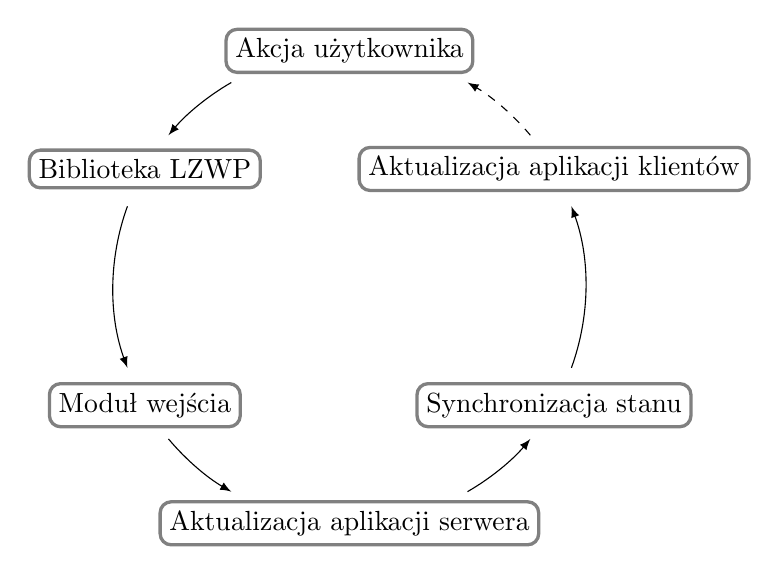
\begin{tikzpicture}[stepstyle/.style={rectangle, 
		rounded corners, draw=gray, very thick,
		text centered, align=center}]
	\def \n {6}
	\def \offset {30}
	\def \radius {3cm}

	\foreach \step [count=\s] in {Akcja użytkownika, Biblioteka LZWP, Moduł wejścia, Aktualizacja aplikacji serwera, Synchronizacja stanu, Aktualizacja aplikacji klientów} {
		\node(\s) [stepstyle] at ({360/\n * (\s) + \offset}:\radius) {\step};
	};
	\foreach \b/\e in {120/140, 160/200, 220/240, 300/320, 340/380} {
		\draw[->, >=latex] ({\b}:\radius)
		arc ({\b}:{\e}:\radius);
	};
		\draw[dashed, ->, >=latex] ({40}:\radius)
		arc ({40}:{60}:\radius);
\end{tikzpicture}
\end{center}
\caption{Diagram kolejności wykonywania modułów przy akcji użytkownika}
\label{fig:diagram-modolow}
\end{figure}



	\section{Zarządzanie pamiecią w aplikacji}
\sectionauthor{Jan Kruczyński}
\label{sec:pamiec}
Ze względu na to, że aplikacja doładowywuje węzły wraz z kolejnymi akcjami użytkownika gdy przemieszcza się on po grafie lub wskazuje na węzły w przestrzeni, musiał zostać opracowany sposób ich usuwania by utrzymać płynność działania. Aby to osiągnąć powstał odzielny kontroler zarządzania pamięcią.

\begin{lstlisting}[caption={Pomocnicze struktury i zmienne kontrolera zarządzania pamięcią}, label=lst:nodePriority]
private List<uint> lowPriorityNodes;%*\label{line:lowPriorityNodes}*)
private List<uint> highPriorityNodes;%*\label{line:highPriorityNodes}*)
public int maxAmountOfNodes;%*\label{line:maxNodes}*)
\end{lstlisting}

Węzły które są załadowane w aplikacji zostały podzielone na dwie kategorie - węzły niskiego priorytetu (\ref{line:lowPriorityNodes}), które są potencjalnmi kandydatami na węzły do usunięcia, oraz wysokiego priorytetu (\ref{line:highPriorityNodes}), których usunąć aktualnie nie można.

Początkowo wszystkie załadowane węzły trafiają do listy niskiego priorytetu. Jeżeli użytkownik dokonuje interakcji z węzłem, to zarówno ten węzeł, jak i wszyscy wyświetlani jego sąsiedzi trafiają do listy wysokiego priorytetu. Jeżeli któryś z tych węzłów znajdował się w liście niskiego priorytetu, jest z niej usuwany i przenoszony na początek listy wysokiego priorytetu.

Funkcjonuje to w taki sposób, aby aplikacja odładowywała w pierwszej kolejności węzły z którymi użytkownik nigdy nie miał interakcji - i dzięki temu nie dostrzegł, że czegoś brakuje. Jednocześnie realizowany jest dodatkowy cel, by ilość wyświetlanych (i przez to przechowywanych w pamięci) węzłów w jednej chwili czasu była stała z dokładnością do kilkunastu sztuk.

Kontroler nasłuchuje zdarzenia załadowania węzła przez aplikację. Gdy takie zdarzenie zostanie wykryte, jeżeli liczba wszytkich węzłów które są wyświetlane w aplikacji nie przekracza maksymalnej dopuszczonej ilości, nie dzieje się nic. Jeżeli ta liczba zostanie przekroczona, odładowuje kilkanaście węzłów z listy niskiego priorytetu (\ref{line:lowPriorityNodes}).

Gdy lista niskiego priorytetu jest pusta, kontroler przerzuca najstarsze węzły z listy wysokiego priorytetu do niskiego (są to węzły z którymi użytkownik prowadził interakcję najdawniej). Gdy użytkownik dokonuje interakcji z węzłem, jest on przerzucany na sam początek listy wysokiego priorytetu.
	\section{Konsola operatora}

	\section{Linia czasu}
\sectionauthor{Mateusz Janicki}
\label{sec:linia-czasu}
Specyfikacja wymagań projektu inżynierskiego zawierała funkcjonalność dotyczącą linii czasu. Wybranie daty miało spowodować wyświetlanie tylko takich węzłów, których data utworzenia była starsza niż wybrana data. Pomogłoby to w przybliżonej wizualizacji, w jak szybki sposób rozrastała się konkretna Wikipedia. Szereg komplikacji spowodował jednak odrzucenie przez nas tej funkcjonalności.

Sterowanie linią czasu miało odbywać się za pomocą drugiego kontrolera. Po wciśnięciu przycisku miał pokazywać się specjalny interfejs ukazujący aktualnie wybraną datę. Można w niej było wybrać, przesuwając joystick w lewo i prawo, miesiąc lub rok, który następnie dałoby się zmieniać przesuwając joystick do góry lub w dół. Zatwierdzenie daty przyciskiem spustu wywoływałoby zmiany w grafie. 

Funkcjonalność nie została zaimplementowana głównie z powodu braku prostej informacji o stworzeniu artykułu w głównie wykorzystywanym przez nas źródle danych, czyli zrzutach baz danych Wikipedii. Istnieją archiwa zawierające kompletną historię edycji artykułów, jednak wielkość tych plików jest nieporównywalnie większa w porównaniu ze zwykłym wykazem stron czy nawet połączeniami pomiędzy stronami. Przetworzenie tych plików tylko po to, aby wydobyć z nich datę pierwszej publikacji strony, jest niewymierna do korzyści wynikających z tej funkcjonalności. 

Innym sposobem wydobycia danych mogłoby być pozyskiwanie tych informacji przy użyciu Wikipedia API. Pomysł ten jednak nie jest wykonalny z powodu ograniczeń, które posiada API. Aby~zdobyć informacje dotyczące każdego artykułu, musielibyśmy wywołać zapytania, których liczba znacznie przewyższa maksymalną dopuszczalną liczbę zapytań dla jednego użytkownika. Przekroczenie tej liczby powoduje zablokowanie adresu IP, z którego pochodziły zapytania i utrudnia dalsze pozyskiwanie danych.

Co więcej, nasza idea linii czasu nie byłaby dokładnym odwzorowaniem stanu Wikipedii w wybranym przez użytkownika czasie. Artykuły i kategorie Wikipedii są bardzo często zmieniane, co implikuje możliwość zmiany połączeń pomiędzy artykułami. Ponadto artykuły i kategorie mogą być także usuwane. Przechowywanie całej historii stron lub stworzenie plików zawierających dokładną historię wszystkich węzłów, jakie kiedykolwiek pojawiły się w Wikipedii, jest niemożliwe na zwykłych komputerach osobistych z powodu zbyt dużej wymaganej przestrzeni na dysku. Nawet jeśli udałoby się je~zapisać, przetwarzanie i wczytywanie takich plików zajęłoby bardzo dużo czasu i spowodowałoby niską responsywność aplikacji. Nasza wersja linii czasu mogłaby być myląca dla nowych użytkowników, którzy mogliby pomyśleć, że przedstawiana jest im dokładna wersja Wikipedii w danym czasie.
	\input{\chapterPath/7_interakcja.tex}
\end{chapter}




\chapter{Konfiguracja i uruchamianie}

\begin{chapter}{Eksperyment}
	\newcommand{\chapterPath}{rozdzialy/6_eksperyment}	
	\sectionauthor{Mateusz Janicki}
Aplikacja została przetestowana na dużej jaskini, po pomyślnym przejściu testów na małej jaskini. Początkowo występowały drobne problemy z synchronizacją, jednak zostały one przez nas rozwiązane. Dopiero na środowisku docelowym istnieje możliwość sprawdzenia poprawności działania efektu 3D przy użyciu okularów zamieszczonych na Rysunku \ref{fig:okulary} oraz intensywniejszej synchronizacji między komputerami. 

\img{\chapterPath/img/okulary-min.JPG}{Okulary umożliwiające widzenie w 3D}{okulary}{.8}

Do testów aplikacji wykorzystane zostały scenariusze użycia opisane w sekcji 2.4. Ostatecznie tylko trzy z pięciu opisanych scenariuszy mogły zostać zrealizowane, ponieważ pozostałe korzystają z niezaimplementowanych i odrzuconych funkcjonalności. Ostatni może zostać zrealizowany tylko częściowo, ponieważ ostatecznie wykorzystywany jest tylko jeden kontroler, więc implementacja systemu zmiany układu sterowania była bezcelowa.

\begin{enumerate}[label=\textbullet]
	\item \textbf{Przejście z węzła “Politechnika Gdańska” do węzła ``Gdańsk''} 
	
Aplikacja została uruchomiona na dużej jaskini. Po włączeniu ukazała się przestrzeń informująca o podstawach sterowania. W celu przejścia do widoku grafu naciśnięty został przycisk 4 na kontrolerze. Spowodowało to odtworzenie krótkiej melodii i pojawienie się węzłów w przestrzeni. Z powodu ograniczonej liczby wyświetlanych węzłów w jednym momencie, znalezienie artykułu ``Politechnika Gdańska'' jest bardzo utrudnione. Znaleziony został on za pomocą konsoli operatora, co znacznie przyspieszyło cały proces. Użytkownik został przeniesiony w momencie wybrania nad węzeł, a na ścianach wokół niego pojawiły się połączenia do innych węzłów. Pojawił się nagłówek z informacją o aktualnie wybranym węźle, ilości połączeń i aktualnie wyświetlanym przedziale ze wszystkich połączeń. Jednocześnie wyświetlane ich było dwanaście, a węzeł “Gdańsk” nie znajdował się w pierwszym zestawie. Zmusiło to użytkownika do przewinięcia dalszych połączeń i szukania docelowego artykułu. Artykuł Gdańsk znaleziony został w siódmym zestawie połączeń. Użytkownik wskazał go kontrolerem, co spowodowało wyświetlenie się nazwy “Gdańsk” i liczby połączeń na nagłówku z informacjami. Odtworzona została także animacja wyświetlająca połączenia wskazywanego artykułu z innymi artykułami, a kolor węzła zmienił się na pomarańczowy. Użytkownik wcisnął przycisk spustu, co skutkowało zaznaczeniem węzła i wyświetlenie jego połączeń.
	\item \textbf{Przejście do artykułu należącego do tej samej kategorii co artykuł ``Jan Matejko''}
	
Po przejściu do widoku grafu ponownie otaczają nas jedynie losowe węzły, a prawdopodobieństwo pojawienia się wśród nich poszukiwanego artykułu jest bardzo niskie. Przed przeprowadzeniem została jednak przygotowana trasa zawierająca najbardziej znanych malarzy w Polsce, a więc wykorzystanie jej jest szybkim sposobem na znalezienie artykułu. Po otwarciu konsoli i przejściu do zakładki ``Routes'' został wciśnięty przycisk ``START'' odpowiadający trasie o nazwie ``Polscy malarze'', co spowodowało przeniesienie użytkownika na artykuł o nazwie ``Józef Chełmoński''. Ponadto zmianie uległa ikona stanu znajdująca się pod nagłówkiem - dopisany do niej został napis ``AUTO'', który świadczy o tym, że jest aktualnie uruchomiona trasa.  Po odczekaniu wyznaczonego w konfiguracji czasu użytkownik jest przenoszony na następny artykuł o nazwie ``Aleksander Gierymski'', a po następnie na poszukiwany przez nas artykuł ``Jan Matejko''. W tym momencie naciśnięty został przycisk 4 powodujący przerwanie trasy oraz zniknięcie napisu ``AUTO'' z ikony stanu. Aby wyświetlić kategorie, należy skierować kontroler na wybrany węzeł i nacisnąć spust. Spowoduje to wyświetlenie zarówno kategorii, do których należy artykuł ``Jan Matejko'', jak i wyświetlenie artykułów, które mają odniesienie do naszego artykułu. Ponadto zmieni się ikona stanu symbolizująca skierowanie w grafie. Poszukiwane kategorie przedstawione są w formie fioletowych figur. Połączenia można przewijać za pomocą przycisków 2 i 3 na kontrolerze. Użytkownik odnalazł kategorię ``Polscy malarze'', wskazał ją i nacisnął spust, zostając przeniesionym na miejsce w grafie gdzie ta kategoria się znajdowała. Ponownie skierował kontroler na węzeł pod sobą i nacisnął spust by powrócić do typu wyświetlanych połączeń prowadzących do artykułów w tej kategorii. Następnie wskazał na artykuł ``Julian Cegliński'' i nacisnął spust.
	\item \textbf{Wyświetlenie pomocy przy sterowaniu i zmiana układu sterowania}
	
Inicjalnie pomoc dotycząca sterowania wyświetlana jest przy starcie aplikacji. Po przejściu do trybu grafu w każdym momencie możliwe jest jednak wyświetlenie pomocy za pomocą przycisku 1 na kontrolerze. Wychodzeniu i wchodzeniu do pomocy za każdym razem towarzyszy efekt dźwiękowy.
\end{enumerate}

Poza wymienionymi wyżej scenariuszami w trakcie eksperymentu sprawdzono również poprawność innych funkcji. Wielokrotnie wykonywano podstawowe akcje dostępne w aplikacji, takie jak pokazywanie pomocy przedstawione na Rysunku \ref{fig:pomoc}, czy wskazywanie artykułów i kategorii w trybie swobodnego lotu po grafie (Rysunek \ref{fig:swobodny_ruch}). 

\img{\chapterPath/img/pomoc-min.JPG}{Ekran pomocy zawierający informacje o sterowaniu}{pomoc}{.8}

\img{\chapterPath/img/swobodny_ruch-min.JPG}{Wskazywanie artykułu w trybie swobodnego lotu}{swobodny_ruch}{.8}

Ponadto poprawnie działa przechodzenie do trybu chodzenia po węzłach. Tryb ten został przedstawiony na Rysunku \ref{fig:artykul} dla zaznaczonego artykułu oraz na Rysunku \ref{fig:kategoria} dla zaznaczonej kategorii. 

\img{\chapterPath/img/artykul_wybrany-min.JPG}{Widok węzła dla wybranego artykułu}{artykul}{.8}

\img{\chapterPath/img/kategoria_wybrana_inne_kategorie-min.JPG}{Widok węzła dla wybranej kategorii}{kategoria}{.8}

Problematyczne okazało się wyświetlanie węzłów na krawędziach ścian jaskini. Ewentualne nieścisłości najbardziej widoczne są w trybie chodzenia po węzłach. Gdy przesuwamy kamerę za pomocą joysticka w lewo i prawo można zauważyć płynne przechodzenie grafik połączonych węzłów ze ściany na ścianę na Rysunku \ref{fig:zachodzenie}, co świadczy o poprawnym działaniu usuwaniu niewidocznych powierzchni (ang. frustum culling). 
Przetestowane zostało również wskazywanie (Rysunek \ref{fig:wskazywanie}) i wybieranie połączeń oraz zmiana trybu wyświetlania. Za każdym razem poprawnie wyświetlana jest ikona informująca o stanie połączeń. Aplikacja zachowuje się poprawnie przy cofaniu i ponawianiu akcji wykonanych przez użytkownika. 

\img{\chapterPath/img/kategoria_wybrana_artykuly-min.JPG}{Wyświetlanie prawidłowego kształtu dla węzła znajdującego się na dwóch ścianach jaskini}{zachodzenie}{.8}

\img{\chapterPath/img/kategoria_wskazywana_wybrana-min.JPG}{Wskazywanie kategorii w widoku węzła}{wskazywanie}{.8}

W momencie włączenia konsoli operatora, pojawia się ikona informująca użytkownika o otwartej konsoli (Rysunek \ref{fig:ikona_konsoli}). Operator może wyszukać dowolny węzeł, a wyniki wyszukiwania aktualizują się w momencie zmiany pola tekstowego (Rysunek \ref{fig:konsola}). Poprawnie działa również funkcjonalność związana z trasami - możliwe jest odtwarzanie i wyłączanie tras. Wszystkim akcjom użytkownika towarzyszy efekt dźwiękowy, co dodatkowo informuje użytkownika o odebraniu sygnału przez aplikację.

\img{\chapterPath/img/ikona_konsoli-min.JPG}{Ikona informująca o otwartej konsoli operatora}{ikona_konsoli}{.8}

\img{\chapterPath/img/konsola-min.JPG}{Konsola operatora na głównym komputerze w dużej jaskini}{konsola}{.8}

Po przeprowadzeniu eksperymentu można stwierdzić, że aplikacja, mimo braku kilku funkcjonalności zawartych w specyfikacji projektu, jest kompletna i użyteczna. Wybrane rozwiązania ułatwiające sterowanie idealnie spełniają swoje zadanie - konsola na głównym komputerze umożliwia przenoszenie na dowolne węzły oraz włączanie predefiniowanych tras. Immersja w aplikacji jest wysoka ze względu na dobrze działający efekt 3D, intuicyjny interfejs i klimatyczną muzykę. Całość powoduje przyjemny odbiór aplikacji i pokazuje nowy pomysł na wykorzystanie jaskini do wizualizacji tworów nie mających reprezentacji w rzeczywistości. 

\end{chapter}

\begin{chapter}{Podsumowanie}
	\newcommand{\chapterPath}{rozdzialy/7_podsumowanie}
	\label{ch:podsumowanie}
	
	Głównym celem pracy inżynierskiej było zaproponowanie rozwiązania nietypowego przedstawienia treści dobrze znanego serwisu Wikipedia i zainteresowania nim potencjalnego użytkownika. Uwaga odbiorcy skierowana jest na strukturę Wikipedii i połączenia między artykułami i kategoriami, a nie ich treść.

	Powstała aplikacja spełnia postawione na początku założenie. Wizualizacja grafu połączeń w przestrzeni pozwala zauważyć istniejące związki między stronami, które trudno zauważyć przeglądając serwis w przeglądarce internetowej. Aplikacja dołączy również do biblioteki materiałów dostępnych do uruchomienia w LZWP i pozwoli zaprezentować różne możliwości jaskini odwiedzającym ją gościom. Większość dostępnych aplikacji odzwierciedla świat rzeczywisty, nasza aplikacja pozwala wprowadzić użytkownika w zupełnie nowy, wygenerowany dynamicznie świat.\\

	\noindent Podział zadań w projekcie oraz przy pisaniu pracy:
	\begin{enumerate}[label=\textbullet]
		\item \textbf{Stanisław Góra:} \newline Podstawa aplikacji, integracja ze środowiskiem jaskini, nadzór nad całością
		\item \textbf{Mikołaj Mirko:} \newline Interfejs użytkownika oraz wygląd aplikacji i programu do tworzenia danych
		\item \textbf{Jan Kruczyński:} \newline Przetwarzanie danych Wikipedii na potrzeby aplikacji, ładowanie węzłów
		\item \textbf{Mateusz Janicki:} \newline Dodatkowe funkcje aplikacji (historia, trasy, wyszukiwanie), skomponowanie i dodanie muzyki
	\end{enumerate}
	
	Projektowanie aplikacji na środowisko jaskini rzeczywistości wirtualnej wiąże się z wieloma trudnościami. Projekt, od rozpoczęcia pracy nad nim, uległ wielu zmianom, co łatwo zauważyć walidując specyfikację napisaną na samym początku z uzyskanym produktem końcowym. Bazowe założenia pozostały jednak bez zmian.

	Wśród zmian w wymaganiach funkcjonalnych (sekcja \ref{sec:wymagania-funkcjonalne}) znajduje się widok treści (podgląd części treści w odrębnym widoku aplikacji). Zrezygnowano z tej funkcjonalności ze względu na aktualny brak dostępu do Internetu w średniej i dużej jaskini. Widoki grafu (swobodnego poruszania się) oraz węzła (podgląd połączeń) zostały zaimplementowane bez większych zmian (sekcja \ref{sec:tryby-widoki}). Funkcjonalność automatycznego i losowego poruszania się po węzłach grafu została zamieniona na możliwość odtwarzania wcześniej przygotowanych tras (sekcja \ref{sec:history}). Celem tej opcji było ułatwienie prezentowania związków między artykułami, lecz w przypadku losowego podróżowania trudno odróżnić interesujące połączenia od wszystkich pozostałych.

	Dużą zmianą wprowadzoną w specyfikacji funkcjonalności była rezygnacja z linii czasu. Ze względu na niewystarczające rozeznanie oraz błędne założenia dotyczące oferowanych przez wybrane źródło danych informacji niemożliwe było zgromadzenie potrzebnych do tej funkcjonalności danych. Szczegółowy opis tej problemowej funkcjonalności został opisany w specjalnej sekcji \ref{sec:linia-czasu}. Względem spisanych wymagań, zmianom uległ również sposób wyświetlania informacji o węzłach, infografiki instruktażowe oraz dodatkowe elementy (sekcja \ref{sec:elementy}). Nagłówek został uszczegółowiony, a pozostałe elementy (takie jak na przykład siatka wspomagająca) dodane w celu zwiększenia użyteczności aplikacji.

	W związku z opisanymi modyfikacjami schemat kontrolera uległ zmianie. Liczba kontrolerów została zredukowana do jednego, a jego przyciski zostały rozplanowane trochę inaczej - tak, aby korzystanie z kontrolera było wygodniejsze. Nowy schemat znajduje się na Rysunku \ref{fig:flystick_new_controls}. To, jak i inne parametry aplikacji zostały, w ramach testów, dostosowane do potrzeb opisanych w wymaganiach jakościowych (sekcja \ref{sec:wymagania-jakosciowe}). Ograniczenie ilości funkcjonalności pozwoliło na skupienie się na pozostałych elementach aplikacji oraz dopracowanie ich.

	Nieprzewidzianym przez nas aspektem pracy stało się wydobycie potrzebnych danych. W pierwotnych założeniach sprowadzało się do pobrania i prostego przetworzenia informacji. Z czasem pojawiały się jednak kolejne problemy (dostępność danych, ich format i rozmiar, oferowane informacje o pojedynczym artykule itp.). Odpowiedzią na skomplikowany proces pozyskiwania i przetwarzania danych jest dodatkowe narzędzie WikiGraph Parser (opisane w rozdziale \ref{ch:dane}). Zostało stworzone w celu ułatwienia generowania plików wejściowych do głównej aplikacji oraz zebraniu algorytmów przetwarzających w jednym miejscu.

	Podczas wykonywania projektu rozwiązane zostało wiele napotkanych problemów. Generowanie plików wykorzystywanych przez aplikację zostało przyspieszone (pomimo, często bardzo dużych, rozmiarów plików), a ich analizowanie przez program uproszczone, wykorzystując maksymalnie skompresowane dane w plikach binarnych. Rozmieszczenie i wizualizacja grafu, a także zastosowane elementy interfejsu sprawnie przekazują niezbędne informacje użytkownikowi, zachowując przy tym prosty, ale zrozumiały wygląd. Integracja elementów jaskini, takich jak okulary i kontrolery, została uproszczona poprzez własny system zarządzania różnymi środowiskami oraz przypisanymi do przycisków i joysticków akcjami. Rozróżnienie środowiska PC do testów na lokalnych komputerach przy pomocy klawiatury i myszki oraz środowiska CAVE do wyświetlania aplikacji w jaskini i sterowania za pomocą kontrolerów niebywale zoptymalizowało nasza pracę nad aplikacją. Problem braku klawiatury wewnątrz jaskini został częściowo rozwiązany poprzez stworzoną konsolę operatora.

	Aplikacja z pewnością może być rozwijana w przyszłości o dodatkowe funkcjonalności, zwiększając jej wartość jako narzędzie analityczne. Uwzględniając w wizualizacji dodatkowe dane, takie jak popularność lub rozmiar treści artykułu, można skupić się na innych zależnościach wewnątrz struktur Wikipedii. Rozwinięcie możliwości sterowania aplikacją o system gestów lub komendy głosowe powinno podwyższyć stopień imersji i ułatwić użytkownikowi odnalezienie się w przestrzeni grafu.

\end{chapter}



\input{meta/Bibliografia.tex}

\renewcommand{\baselinestretch}{1.0}\normalsize
\addcontentsline{toc}{chapter}{\listfigurename}
\listoffigures

\addcontentsline{toc}{chapter}{\listtablename}
\listoftables
\renewcommand{\baselinestretch}{1.3}\normalsize

\end{document}
